\documentclass[a4paper, 15pt, oneside]{book}
\usepackage[italian]{babel}
\usepackage[utf8]{inputenc}
\usepackage[a4paper,top=2.5cm,bottom=2.5cm,left=2cm,right=2cm]{geometry}
\usepackage{amssymb}
\usepackage{amsthm}
\usepackage{graphics}
\usepackage{amsfonts}
\usepackage{amsmath}
\usepackage{amstext}
\usepackage{engrec}
\usepackage{rotating}
\usepackage[safe,extra]{tipa}
\usepackage{multirow}
\usepackage{hyperref}
\usepackage{enumerate}
\usepackage{braket}
\usepackage{marginnote}
\usepackage{pgfplots}
\usepackage{cancel}
\usepackage{polynom}
\usepackage{booktabs}
\usepackage{enumitem}
\usepackage{algorithm}
\usepackage{algpseudocode}
\usepackage{framed}
\usepackage{pdfpages}
\usepackage{pgfplots}
\usepackage{fancyhdr}
\usepackage{caption}
\usepackage{subcaption}
\usepackage{setspace}
\usepackage{hyperref}
\pagestyle{fancy}
\fancyhead[L,RO]{\slshape \rightmark}
\fancyfoot[C]{\thepage}

\title{Metodi per il calcolo scientifico}
\author{Tommaso Ferrario (\href{https://github.com/TommasoFerrario18}{@TommasoFerrario18}) \\\\
Telemaco Terzi (\href{https://github.com/Tezze2001}{@Tezze2001}) \\\\
Simone Vendramini (\href{https://github.com/simone-vendramini}{@simone-vendramini})}
\date{Marzo 2024}

\pgfplotsset{compat=1.13}

\begin{document}

\maketitle
\newtheorem{teorema}{Teorema}
\newtheorem{dimostrazione}{Dimostrazione}
\newtheorem{definizione}{Definizione}
\newtheorem{esempio}{Esempio}
\newtheorem{osservazione}{Osservazione}
\newtheorem{nota}{Nota}
\newtheorem{corollario}{Corollario}
\tableofcontents
\renewcommand{\chaptermark}[1]{
    \markboth{\chaptername
        \ \thechapter.\ #1}{}}
\renewcommand{\sectionmark}[1]{\markright{\thesection.\ #1}}

\chapter*{Introduction}
\textbf{Deep Learning} is a subset of machine learning that is concerned with 
neural networks that are use to learn underlying features in data.

In general, we can define machine learning as a program that starting from the 
input and the output of a system, learns the rules that govern the system. In 
order to obtain high performance, machine learning algorithms depends heavily on 
the \textbf{representation} of the data. Representation is therefore the fundamental, 
and many artificial intelligence tasks can be solved by designing the right set of features.

The most difference between Deep ML and ML is that, the first one try to learn an
efficient representation of data and than use it to train a learn model. The latter 
one use a representation of data specified by an expert to train a learn model.

Deep Learning use neural networks with many layers of activity vectors as 
representations and learning the connection strengths between that give rise to 
these vectors by following the stochastic gradient of an objective function that
measures how well the network is performing.

So, the key ingredient of deep learning is \textbf{Depth}. There are two main 
ways to measure the depth of a model:
\begin{enumerate}
    \item in terms of depth of the graph describing how concepts are related to
        each other.
    \item in terms of number of sequential instructions that must be executed to 
        evaluate the architecture. This can be influenced by the choice of basic 
        functions used.
\end{enumerate}

One solution to the problem of feature representation is to use machine learning
not only to find the mapping between input and output, but also to find the
representation itself. This approach is called \textbf{Representation Learning}.
The goal of this task is to identify the \textit{factor of variations} that 
explain the observed data. The goal of this task is to identify the factor of 
variations that explain the observed data.

The most common example of representation learning is the use of autoencoders.

A key part of representation learning consists in the \textbf{distributed 
    representation}, which means a many to many relationship between two types
of representation:
\begin{itemize}
    \item Each concept is represented by many neurons.
    \item Each neuron participates in the representation of many concepts.
\end{itemize}

Deep learning solves this central problem in representation learning by introducing
representations that are expressed in therms of other, simpler representations.
An example is bunch of letters form words, sets of words form phrases.

\chapter{Ripasso Algebra Lineare}
\begin{definizione} [\textbf{Spazio vettoriale}]
    Un insieme $V$ si dice \textbf{spazio vettoriale} se sono definite su $V$ due
    operazioni che godono di particolari proprietà:
    \begin{itemize}
        \item \textbf{Somma}: $+: V \times V \rightarrow V$
        \item \textbf{Prodotto per uno scalare}: $\cdot : V \times \mathbb{R} \rightarrow V$
    \end{itemize}
\end{definizione}

Le operazioni dello spazio vettoriale godono di alcune proprietà:
\begin{itemize}
    \item \textbf{Somma}:
          \begin{itemize}
              \item \textbf{Commutativa}: $\forall u,v \in V, u+v = v+u$
                    \begin{proof}
                        $\forall u,v \in V:$
                        $$ u+v = \left[\begin{array}{c}
                                    u_1 \\u_2\\ \vdots \\u_n
                                \end{array}\right] + \left[\begin{array}{c}
                                    v_1 \\v_2\\\vdots\\v_n
                                \end{array}\right] = \left[\begin{array}{c}
                                    u_1 + v_1 \\u_2 + v_2\\\vdots\\u_n+v_n
                                \end{array}\right] = \left[\begin{array}{c}
                                    v_1 + u_1 \\v_2 + u_2\\\vdots\\v_n+u_n
                                \end{array}\right] = \left[\begin{array}{c}
                                    v_1 \\v_2\\\vdots\\v_n
                                \end{array}\right] + \left[\begin{array}{c}
                                    u_1 \\u_2 \\\vdots\\u_n
                                \end{array}\right] = v+ u$$
                    \end{proof}
              \item \textbf{Associativa}: $\forall u,v,z \in V, (u+v)+z = v+(u+z)$
                    La dimostrazione si può fare facilmente utilizzando sempre la proprietà
                    associativa della somma tra scalari.
              \item \textbf{Esistenza dell'elemento neutro}: $\exists 0 \in V: 0+v = v,
                        \forall v\in V$
              \item $\forall u \in V, \exists w\in V \text{ unico}: u+w=0$
          \end{itemize}
    \item \textbf{Prodotto per uno scalare}:
          \begin{itemize}
              \item \textbf{Distributivo rispetto alla somma}: $\forall u,v \in
                        V, \forall \lambda \in \mathbb{R}, \lambda(u+v) = \lambda
                        u+\lambda v$
              \item \textbf{Distributivo rispetto alla somma tra scalari}:
                    $\forall u \in V, \forall \lambda,\mu\in \mathbb{R}: (\lambda +
                        \mu)u = \lambda \cdot u + \mu \cdot u$
              \item \textbf{Associativo rispetto al prodotto tra scalari}:
                    $\forall u \in V, \forall \lambda,\mu\in \mathbb{R}: (\lambda \cdot
                        \mu)u = \lambda \cdot (\mu \cdot u)$
              \item \textbf{Esistenza dell'elemento neutro}: $\exists 1 \in
                        \mathbb{R}:1\cdot v = v, \forall v\in V$
          \end{itemize}
\end{itemize}
\begin{esempio}
    Un esempio di spazio vettoriale è $V\in \mathbb{R}^n$
\end{esempio}
\begin{definizione} [\textbf{Prodotto scalare}]
    Sia $V$ uno spazio vettoriale, definiremo il \textbf{prodotto scalare} è un'operazione
    che a due elementi di $V$ associa un valore reale, $(\cdot, \cdot):V\times V
        \rightarrow \mathbb{R}$.Tale operazione soddisfa le seguenti proprietà:
    \begin{itemize}
        \item \textbf{Simmetrica}: $\forall u,v \in V, (u,v) = (v,u)$
        \item \textbf{Bi-lineare}: $\forall v_1,v_2,w \in V,\forall\alpha_1,
                  \alpha_2 \in \mathbb{R}:(\alpha_1v_1+\alpha_2v_2, w) =
                  \alpha_1(v_1, w) + \alpha_2(v_2, w)$
        \item $\forall v \in V, v\ne 0: (v,v) \ge 0$
    \end{itemize}
\end{definizione}
\begin{definizione} [\textbf{Norma di un vettore}]
    Sia $V$ uno spazio vettoriale, definiremo la \textbf{norma di un vettore} è
    un'operazione che a un elemento di $V$ associa un valore reale, $\|\cdot\|:
        V \rightarrow \mathbb{R}$. Tale operazione soddisfa le seguenti proprietà:
    \begin{itemize}
        \item \textbf{scalabilità}: $\forall v \in V,\forall \alpha \in \mathbb{R}:
                  \|\alpha v\| = |\alpha | \|v\|$
        \item \textbf{disuguaglianza triangolare}: $\forall v,w \in V: \|v+w\|
                  \le \|v\| + \|w\|$
        \item $\forall v \in V, v\ne 0: \|v\| > 0\implies \|0\| = 0$
    \end{itemize}
\end{definizione}
La definizione e le proprietà derivano dalla nota successiva
\begin{nota} [\textbf{Norma indotta dal prodotto scalare}]
    Sia $V$ uno spazio vettoriale in cui è definito un prodotto scalare allora è
    possibile calcolare la norma da $(\cdot, \cdot)$
    \begin{equation}
        \|v\| = \sqrt{(v,v)}  \equiv \|v\|_2
    \end{equation}
    Tale norma viene chiamata \textbf{norma indotta dal prodotto scalare }
\end{nota}
\begin{nota}
    Esistono diverse norme oltre alla $2$:
    \begin{itemize}
        \item $\|v\|_2 = \sqrt{\sum_{i=1}^{N}v_i^2} = \|v-0\|$
        \item $\|v\|_1 = \sum_{i=1}^{N}|v_i|$
        \item $\|v\|_\infty = \max_{i= 1\dots n}|v_i|$
    \end{itemize}
\end{nota}
La norma euclidea ($\|\cdot\|_2$) è utile per calcolare la distanza di vettori
perché $\|v\|_2$ calcola la distanza di $v$ da $0$, mentre $\|v-w\|_2$ calcola
la distanza tra $v$ e $w$.

Quindi dato un prodotto scalare possiamo sempre definire la norma, ma non possiamo
dire il contrario.
\begin{nota}
    La norma ha una proprietà indotta dalla sua definizione e dalle sue proprietà,
    $\forall v,w \in V$
    \begin{equation*}
        \|v\| -\|w\| \le \|v-w\|
    \end{equation*}
\end{nota}
Possiamo definire anche le norme per le matrici $V\in \mathbb{R}^{r\times c}$:
\begin{itemize}
    \item $\|A\|_F = \sqrt{\sum_{i,j} |a_{i,j}|^2}$
    \item $\|A\|_1 = \max_{i=1\dots r}{\sum_{j=1}^{c} |a_{i,j}|}$
    \item $\|A\|_\infty = \max_{j=1\dots c}{\sum_{i=1}^{r} |a_{i,j}|}$
\end{itemize}

Altre operazioni utili per gli spazi vettoriali, generalmente per vettori e matrici, è
la \textbf{trasposizione}.
\begin{equation}
    A=\left[\begin{array}{ccc}
            a & b & c \\
            d & e & f
        \end{array}\right]\in \mathbb{R}^{2\times3},  A^t = \left[\begin{array}{cc}
            a & d \\
            b & e \\
            c & f
        \end{array}\right]\in \mathbb{R}^{3\times2}
\end{equation}
Il problema di questa operazione è che non è \textbf{chiusa} ovvero non rimane
nello stesso spazio.

In aggiunta si ha \textbf{prodotto tra matrici e vettori}. Dati $A\in \mathbb{R}^{r\times c}$
e $v\in \mathbb{R}^{c}$ si ha:
\begin{equation*}
    Av = \left[\begin{array}{cccc}
            a_{11} & a_{12} & \cdots & a_{1c} \\
            a_{21} & a_{22} & \cdots & a_{2c} \\
            \vdots & \vdots & \dots  & \vdots \\
            a_{r1} & a_{r2} & \cdots & a_{rc}
        \end{array}\right] \left[\begin{array}{c}
            v_1 \\v_2\\\vdots\\v_c
        \end{array}\right] = \left[\begin{array}{c}
            a_{11}v_1+a_{12}v_2+\cdots a_{1c}v_c \\
            a_{21}v_1+a_{22}v_2+\cdots a_{2c}v_c \\
            \vdots                               \\
            a_{r1}v_1+a_{r2}v_2+\cdots a_{rc}v_c \\
        \end{array}\right]
\end{equation*}
Questa operazione è vincolata dal fatto che la matrice e il vettore devono
essere compatibili, le colonne della matrice devono essere uguali alle righe del
vettore. Inoltre abbiamo anche l'operazione di \textbf{prodotto matrice-matrice}.
Sia $A\in \mathbb{R}^{3\times 2}, B\in \mathbb{R}^{2\times 4}$
\begin{equation*}
    AB = \left[\begin{array}{cc}
            a & b \\
            c & d \\
            e & f
        \end{array}\right]\left[\begin{array}{cccc}
            g & h & i & l \\
            m & n & o & p \\
        \end{array}\right] = \left[\begin{array}{cccc}
            ag+bm & ah+bn & ai+bo & al+bp \\
            cg+dm & ch+dn & ci+do & cl+bp \\
            eg+fm & eh+fn & ei+fo & el+fp \\
        \end{array}\right]
\end{equation*}
Anche questa operazione è vincolante perché può essere effettuata solo quando la
prima matrice ha il numero di colonne uguale al numero di righe della seconda.
Inoltre la commutazione non sempre è fattibile perché potrebbero non essere
compatibili e in generale \textbf{non} è commutativa. La soluzione del prodotto
può essere conosciuta in anticipato quando tra i fattori del prodotto si hanno
matrici particolari.
\begin{definizione}[\textbf{Matrice sparsa}]
    Se una matrice $A\in \mathbb{R}^{n \times m}$ ha poche entrate diverse da $0$
    allora si dice \textbf{sparsa}.
\end{definizione}

Supponiamo di avere $A\in \mathbb{R}^{3\times 3}$ sparsa e $B\in \mathbb{R}^{3\times3}$
\begin{equation*}
    \left[\begin{array}{ccc}
            1 & 0 & 0 \\
            0 & 0 & 1 \\
            0 & 1 & 0
        \end{array}\right]  \left[\begin{array}{ccc}
            a & b & c \\
            e & f & g \\
            h & i & l
        \end{array}\right] = \left[\begin{array}{ccc}
            a & b & c \\
            h & i & l \\
            e & f & g \\
        \end{array}\right]
\end{equation*}
In questo caso si ha uno scambio della seconda riga con la terza.
\begin{equation*}
    \left[\begin{array}{ccc}
            a & b & c \\
            e & f & g \\
            h & i & l
        \end{array}\right] \left[\begin{array}{ccc}
            1 & 0 & 0 \\
            0 & 0 & 1 \\
            0 & 1 & 0
        \end{array}\right] = \left[\begin{array}{ccc}
            a & c & b \\
            e & g & f \\
            h & l & i \\
        \end{array}\right]
\end{equation*}
In questo caso abbiamo fatto lo scambio della seconda colonna con la terza.
Quindi pre o post moltiplicare una matrice $B$ per una matrice $A$ composta da
un solo uno per ogni riga/colonna ha l'effetto di scambiare le corrispondenti
righe/colonne.
\begin{definizione}[\textbf{Matrice di permutazione}]
    Matrici $A \in \mathbb{R}^{n\times n}$ che permettono di effettuare scambi di
    righe o colonne sono dette \textbf{matrici di permutazione}.
\end{definizione}
Queste sono utili per risolvere i sistemi lineari e permettono di velocizzare le
operazioni di calcolo.

Supponiamo ora di considerare il seguente esempio:
\begin{equation*}
    \left[\begin{array}{ccc}
            1 & 0 & 0 \\
            0 & 1 & 0 \\
            0 & 0 & 1
        \end{array}\right]  \left[\begin{array}{ccc}
            a & b & c \\
            d & e & f \\
            g & h & i
        \end{array}\right] = \left[\begin{array}{ccc}
            a    & b    & c    \\
            2a+d & 2f+e & 2c+f \\
            g    & h    & i    \\
        \end{array}\right]
\end{equation*}
Da esso, possiamo affermare che meno coefficienti ha la matrice più è facile
capire come sarà la matrice risultante.

In aggiunta possiamo trasformare un sistema di equazioni lineari in un prodotto
tra matrice e vettore ($Ax+b=0\equiv a_1x_1+a_2x_2+\dots a_n x_n = b$). Dove $a_i$
è il vettore dei coefficienti della variabile $x_i$. Questa rappresentazione dei
sistemi permette di risolverli facilmente utilizzando dei metodi specifici per le
tipologie di matrici particolari, fondamentale sarà quindi riconoscere la tipologia
di matrici.

Altre matrici particolari sono quelle \textbf{triangolari inferiori/superiori}
che sono utili per risolvere i sistemi lineari usando il metodo di sostituzioni.
\begin{esempio}
    Esempio di matrice triangolare inferiore
    \begin{equation*}
        \left[\begin{array}{ccc}
                1 & 0 & 0 \\
                2 & 1 & 0 \\
                1 & 1 & 1
            \end{array}\right]
    \end{equation*}
\end{esempio}
\begin{esempio}
    Esempio di matrice triangolare superiore
    \begin{equation*}
        \left[\begin{array}{ccc}
                1 & 1 & 1 \\
                2 & 1 & 0 \\
                1 & 0 & 0 \\
            \end{array}\right]
    \end{equation*}
\end{esempio}

Un'altra matrice utile è quella \textbf{simmetrica}, ovvero una matrice quadrata
tale che $a_{ij} = a_{ji}$.

Un altro tipo di matrice particolare è quella dei sistemi con moltissime variabili,
moltissime equazioni ciascuna con poche variabili, quindi si parlerà di
\textbf{sistema lineare sparsi}, ovvero con un numero minore del $10\%$ di
entrate con valori diversi da $0$. Sarà importante trovare un modo per salvare i
valori delle matrici in modo efficiente.

Un operazione utile per la risoluzione dei sistemi lineari è il \textbf{determinante},
ovvero $det(A): \mathbb{R}^{n\times n} \rightarrow \mathbb{R}$. Il determinante
è utile per scoprire la presenza di soluzioni e se sono uniche.
\begin{equation}
    det(A) = \sum_{j = 1}^{n}(-1)^{i+j} \, a_{ij} \, det(A_{ij})
\end{equation}
\chapter{Analisi Numerica}
\section{Introduzione}
In questo capitolo verranno presentate alcune tecniche per la risoluzione dei
sistemi lineari e il concetto di \textbf{numero di condizionamento}.

Lo sviluppo di un algoritmo di risoluzione di sistemi lineari deve considerare
tre fattori:
\begin{enumerate}
    \item \textbf{Memoria}: l'algoritmo deve richiedere un quantitativo ridotto
          di memoria.
    \item \textbf{Velocità}: l'algoritmo deve essere molto veloce.
    \item \textbf{Precisione}: vogliamo ottenere una soluzione più vicina possibile
          a quella reale.
\end{enumerate}
\subsection{Gestione di Matrici e Vettori}
A livello di programmazione, i vettori possono essere salvati utilizzando
aree congiunte di memoria (array). Mentre, per quanto riguarda le matrici, si
possono salvare in array secondo diverse filosofie:
\begin{itemize}
    \item \textbf{Row Major}: si salvano le righe una dopo l'altra.
          \begin{figure}[!ht]
              \centering
              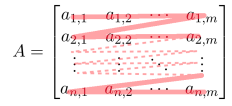
\includegraphics[width=0.25\textwidth]{./img/AnalisiNumerica/RowMajor.png}
              \caption{Esempio di salvataggio di una matrice in Row Major}
          \end{figure}
    \item \textbf{Column Major}: si salvano le colonne una dopo l'altra.
          \begin{figure}[!ht]
              \centering
              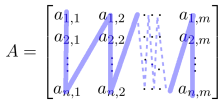
\includegraphics[width=0.25\textwidth]{./img/AnalisiNumerica/ColumnMajor.png}
              \caption{Esempio di salvataggio di una matrice in Column Major}
          \end{figure}
\end{itemize}

Per salvare una matrice \textbf{sparsa} viene sempre salvata come collezione di
tuple $\langle i, \, j,\, val\rangle$. Con questa rappresentazione, anche nota
come \textbf{formato sparso}, ogni qualvolta si effettua un'operazione tra matrici
sparse si trasformano in matrici normali e si applica l'operazione.
\subsection{Gestione Errori}
L'algoritmo creato deve essere valutato in base a quanto è vicino il risultato
restituito rispetto a quello corretto. Questo deve essere fatto in quanto
i risultati sono spesso forniti come numeri floating point e quindi soggetti
a errori di approssimazione.

\begin{definizione}[\textbf{Errore assoluto}]
    Sia $\stackrel{\sim}{\textbf{x}}$ la soluzione approssimata di un sistema
    lineare $A\textbf{x} = \textbf{b}$ e sia $x$ la soluzione corretta, allora
    l'\textbf{errore assoluto} è definito come:
    \begin{equation}
        \epsilon = \|\stackrel{\sim}{\textbf{x}} - \textbf{x}\|
    \end{equation}
    dove $\|\cdot\|$ è una qualsiasi norma fra due vettori.
\end{definizione}
\begin{definizione}[\textbf{Errore relativo}]
    Sia $\stackrel{\sim}{\textbf{x}}$ la soluzione approssimata di un sistema
    lineare $A\textbf{x} = \textbf{b}$ e sia $x$ la soluzione corretta, allora
    l'\textbf{errore relativo} è definito come:
    \begin{equation}
        \epsilon = \frac{\|\stackrel{\sim}{\textbf{x}} - \textbf{x}\|}{\|\textbf{x}\|}
    \end{equation}
    dove $\|\cdot\|$ è una qualsiasi norma fra due vettori.
\end{definizione}

Il problema è conoscere la soluzione esatta del sistema per calcolare l'errore.
Un modo per ottenere la soluzione esatta possiamo inizializzare un vettore $x$ in modo
randomico. In questo modo si calcola il vettore $b =A\cdot x $ e successivamente
si utilizza algoritmo di risoluzione di sistemi per risolvere il seguente
sistema $A\cdot \stackrel{\sim}{x} = b$. In questo modo $x$ è la soluzione esatta
mentre  $\stackrel{\sim}{x}$ è la soluzione approssimata. Ovviamente questa non è
la soluzione reale, ma ci interessa principalmente sapere se è risolvibile il sistema
e con che errore. Questo è determinato dalla matrice $A$ ma non dal vettore dei
termini noti $b$, per questo ci si calcola un vettore $b$ dipendente dalla soluzione
"esatta" randomica.
\begin{teorema}\label{teo:NormeEquivalenti}
    Il comportamento delle norme di vettori in $\mathbb{R}^n$ è equivalente. ossia
    preso un vettore $x\in \mathbb{R}^n$, $\exists c_1,c_2\in \mathbb{R}$ tali che:
    \begin{equation}
        c_1\|x\|_p < \|x\|_q < c_2\|x\|_p
    \end{equation}
\end{teorema}
Il teorema \ref{teo:NormeEquivalenti} ci dice che le norme a meno di alcuni
fattori moltiplicativi restituiscono gli stessi risultati.
\subsection{Velocità}
Come precedentemente detto, un aspetto importante è la velocità dell'algoritmo.
Per calcolare questo parametro dobbiamo contare il numero di operazioni che
effettuiamo, nello specifico si andrà ad utilizzare la complessità asintotica.

Analizziamo ora le velocità delle diverse operazioni:
\begin{itemize}
    \item \textbf{Prodotto Scalare}: sia $(x,y) = \sum_{i=1}^n x_iy_i$ corrisponde
          ad effettuare $n$ prodotti e $n-1$ somme, quindi si ha $n + n - 1 = 2
              n -1 \in \mathcal{O}(n)$
    \item \textbf{Norma di un vettore}: sia $\|x\| = \sqrt{\sum_{i=1}^n x_i^2}$
          corrisponde ad effettuare $n$ prodotti e $n-1$ somme, quindi si ha
          $n + n - 1 = 2n -1 \in \mathcal{O}(n)$
    \item \textbf{Prodotto Matrice-Vettore}: siano $A\in \mathbb{R}^{r\times c}$
          e $v\in \mathbb{R}^c$ allora $Av\in \mathcal{O} (rc) = \mathcal{O}(n^2)$
    \item \textbf{prodotto Matrice-Matrice}: siano $A,B\in \mathbb{R}^{n\times n}$
          allora $AB\in \mathcal{O} (n \cdot n \cdot n) = \mathcal{O} (n^3)$
    \item \textbf{Determinate}: sia $A\in \mathbb{R}^{n\times n}$ allora
          $det(A) \in \mathcal{O}(n!)$.
\end{itemize}
\section{Numero di Condizionamento}
Sappiamo che presa una matrice $A \in \mathbb{R}^{n \times n}$ e un vettore $b
    \in \mathbb{R}^n$ diverso dal vettore nullo, il sistema lineare $A \textbf{x} =
    \textbf{b}$ ammette soluzione se e soltanto se $det(A) \neq 0$.

Purtroppo quando si risolvono i sistemi lineari al calcolatore subentrano una
serie di altri fattori che influenzano il modo in cui si risolve il sistema e,
di conseguenza, la soluzione stessa. Questi fattori sono dovuti essenzialmente
alla rappresentazione dei numeri e agli errori di arrotondamento nelle operazioni.

Oltre a ciò, analizzando le velocità delle operazioni, si può notare che il
calcolo del determinante è molto complesso, quindi non è possibile utilizzarlo
per capire se un sistema è complesso da risolvere.

Per ovviare a questo problema, si introduce il concetto di \textbf{numero di
    condizionamento} calcolato su una matrice. Se tale valore è alto allora il
sistema è complesso da risolvere.
\begin{definizione}[\textbf{Numero di Condizionamento}]
    Presa una matrice $A \in \mathbb{R}^{n \times n}$, il \textbf{numero di
        condizionamento} è definito come:
    \begin{equation}
        cond(A) = \|\lambda_{max}\| \cdot \|\lambda_{min}\|
    \end{equation}
    dove $\lambda_{max}$ e $\lambda_{min}$ sono rispettivamente il massimo e il
    minimo autovalore della matrice $A$ in modulo.
\end{definizione}
Per definizione il numero di condizionamento è una quantità maggiore di $1$.
Vedremo che più questa quantità è vicino a $1$ più il sistema sarà facile da
risolvere numericamente, ossia risente meno dell'algebra di macchina. Di contro
più grande è questa quantità più il sistema sarà risolto “male”.
\begin{esempio}[Numero di Condizionamento di una Matrice di Hillbert]
    Prendiamo una matrice $H \in \mathbb{R}^{n \times n}$ definita nel seguente modo:
    \begin{equation*}
        H_{ij}=\frac{1}{1+i+j}
    \end{equation*}
    Questa matrice è nota con il nome di matrice di Hillbert ed è il classico
    esempio di matrice mal condizionata.
\end{esempio}
\section{Metodi per risolvere i sistemi}
Esistono due tipologie di metodi per la risoluzione dei sistemi lineari:
\begin{itemize}
    \item \textbf{Metodi diretti}: si effettuano delle operazioni per ottenere
          in automatico la soluzione dei sistemi.
    \item \textbf{Metodi iterativi}: sono procedure che creano una sequenza di
          vettori soluzioni che si avvicinano sempre di più alla soluzione esatta
          $\|x -\stackrel{\sim}{x}\|\rightarrow 0$ oppure si calcola $\frac{\|x
                  -\stackrel{\sim}{x}\|}{\|A\stackrel{\sim}{x} - b\|}\rightarrow 0$.
\end{itemize}
\section{Metodi diretti}
Partiamo analizzando il caso più semplice, ovvero che il sistema ammette un unica
soluzione. L'assunzione principale è che le matrici abbiano determinante diverso
da $0$.
\subsection{Sostituzione all'indietro}
Il metodo della \textbf{sostituzione all'indietro} è il metodo più efficiente per
risolvere sistemi composti da una matrice quadrata triangolare superiore.
\begin{equation}
    \begin{cases}
        u_{11}x_1 + u_{12} x_2 + \dots + u_{1n} x_n= b_1 \\
        u_{22}x_2 + u_{23} x_3 + \dots + u_{2n} x_n= b_2 \\
        \vdots                                           \\
        u_{nn}x_n = b_n                                  \\
    \end{cases} \iff \left[\begin{array}{cccc}
            u_{11} & u_{12} & \dots  & u_{1n} \\
            0      & u_{22} & \dots  & u_{2n} \\
            \vdots & \ddots & \ddots & \vdots \\
            0      & \dots  & 0      & u_{nn}
        \end{array} \right] \cdot x = \left[\begin{array}{c}
            b_1    \\
            b_2    \\
            \vdots \\
            b_n
        \end{array}\right]
\end{equation}
A livello computazione è semplice testare se la matrice è compatibile con questo
metodo.

Una volta effettuata la verifica, il metodo coincide con il risolvere il sistema
per sostituzione.
\begin{nota}
    Bisogna stare attenti che la diagonale non contenga $0$ perché ogni volta
    si divide per un termine sulla diagonale.
\end{nota}

Sotto le ipotesi di matrice triangolare superiore possiamo calcolare facilmente
il determinante, basta calcolare il prodotto dei termini sulla diagonale, questo
ci dice che esiste una sola soluzione se il determinante è diverso da $0$
($\mathcal{O}(n)$). In aggiunta, questo ci assicura che la diagonale non contiene $0$.

La complessità dell'algoritmo sarà:
\begin{equation*}
    \#\_righe \cdot \#operazioni\_max\_riga = n \cdot (n - 1 + n - 1 + 1) = n
    \cdot (2n - 1) = \mathcal{O}(n^2)
\end{equation*}
\begin{nota}
    Dove il numero massimo di operazioni per riga è $n - 1$ differenze, $n - 1$
    prodotti e $1$ divisione perché nella prima riga si ha:
    \begin{equation*}
        x_1 = \frac{(b_1 - u_{12} x_2 - u_{13}x_3 - \dots - x_{1n} x_n)}{u_{11}}
    \end{equation*}
\end{nota}
Ogni singola operazione per riga si può ricavare iterativamente nel seguente modo
\begin{equation*}
    x_{n-i} = \frac{(b_i-(u_{n-i},x))}{u_{ii}}
\end{equation*}
Con $x$ inizializzato a tutti $0$ tranne la cella $n$ che sarà inizializzata a:
\begin{equation*}
    x_n = \frac{b_n}{u_{nn}}
\end{equation*}
Mentre $i$ è inizializzato a $1$, ad ogni iterazione si utilizza il vettore $x$
aggiornato nell'iterazione precedente. Al termine si ottiene una soluzione per il
sistema.
\begin{nota}
    Questo metodo può essere utilizzato anche per i sistemi lineari descritti da
    una matrice triangolare inferiore. In questo caso prima sarà necessario
    trasformare la matrice in una matrice triangolare superiore. Questo si può
    fare riordinando le righe della matrice e specchiando la matrice la colonna
    centrale. Lo stesso ragionamento si può applicare anche per matrici diagonali
    rispetto alla antidiagonale.
\end{nota}
\begin{nota}
    Ricorda che quando si effettua un permutazione delle righe il sistema rimane
    invariato, al contrario se effettuassi una permutazione delle colonne allora
    sto cambiando le incognite, perciò dovrei cambiare anche il vettore delle
    incognite se io volessi mantenere lo stesso sistema.
\end{nota}
\subsection{Trasformazioni di Gau$\Beta$}
Per risolvere sistemi a cui sono associate matrici che non sono triangolari,
come quella riportata di seguito, non possiamo più pensare all'algoritmo di
sostituzione all'indietro.
\begin{equation}
    \begin{cases}
        a_{11}x_1 + a_{12} x_2 + \dots + a_{1n} x_n= b_1 \\
        a_{21}x_1 + a_{22} x_2 + \dots + a_{2n} x_n= b_2 \\
        \vdots                                           \\
        a_{n1}x_1 + a_{n2} x_2 + \dots + a_{nn} x_n= b_n \\
    \end{cases}
\end{equation}

Per sistemi generici di $n$ equazioni in $n$ incognite i metodi di risoluzione
sono diversi. L'algoritmo di eliminazione di Gauss si basa sul fatto che, preso
un sistema lineare è possibile modificare le sue equazioni in modo da ottenere
un sistema lineare equivalente, ossia che ha la stessa soluzione del sistema di
partenza. Questo si può fare utilizzando le seguenti trasformazioni:
\begin{itemize}
    \item \textbf{Scambiare le righe}
    \item \textbf{Riduzione}: Sostituire una riga con una combinazione lineare di
          se stessa con un'altra
\end{itemize}
Successivamente si eseguirà sul sistema equivalente il metodo di risoluzione per
sostituzione all'indietro.

Per effettuare riduzione della matrice associata al sistema ad una matrice
triangolare superiore, applichiamo una serie di trasformazioni in modo da azzerare
i coefficienti al di sotto della diagonale. L'applicazioni delle trasformazioni
deve essere effettuata sulle righe della \textbf{augmented matrix form}, ovvero
la matrice del sistema con l'aggiunta del vettore dei termini noti a destra dei
coefficienti delle incognite.
\begin{definizione}[\textbf{Pivot}]
    Il termine che si sceglie per procedere con la sostituzione di tutte le
    equazioni del sistema lineare viene chiamato \textbf{pivot}.
\end{definizione}
\begin{nota}
    Sotto l'ipotesi di sistema risolubile (determinante non nullo) allora il metodo
    di Gau$\Beta$ convergerà ad una matrice triangolare superiore. Quindi non
    rischio di sostituire una riga con un coefficiente moltiplicatore di un'altra
    riga avente denominatore nullo. Quindi, quando abbiamo una riga che ha il
    coefficiente sulla diagonale pari a $0$ allora siamo sicuri che troveremo
    un'altra riga con un coefficiente non nullo.
\end{nota}
\begin{osservazione}
    Durante tutto il procedimento osserviamo che la scelta del pivot e quindi
    del moltiplicatore dipende solamente dalla matrice A e non dal termine noto.
    Il termine noto viene sempre e solo aggiornato in modo da ottenere un sistema
    lineare equivalente!
\end{osservazione}

Calcoliamo ora la complessità di tale algoritmo. Il peggiore dei casi è quando
effettuiamo la prima riduzione. Nello specifico, per essa dobbiamo calcolare:
\begin{equation*}
    R_i = R_i - \frac{a_{11}\cdot a_{a_i1}}{a_{11}} R_1
\end{equation*}
Queste operazioni sono $n + 1$ differenze, $n + 1$ prodotti e $1$ divisione. Quindi
per una riga sono necessarie $1 + n + 1 + n + 1 = 2 n + 3 =\mathcal{O}(n)$.
Questo deve essere ripetuto per $n - 1$ volte per azzerare la prima colonna,
in termini di complessità asintotica $\mathcal{O}(n^2)$. Dal momento che dobbiamo
ridurre un totale di $n-1$ colonne quindi si ha $\mathcal{O}(n^2\cdot n) = \mathcal{O}(n^3)$.
Attualmente non stiamo risolvendo il sistema, bensì lo stiamo solo trasformando,
per anche risolverlo impiegheremo  $\mathcal{O}(n^3+ n^2) =\mathcal{O}(n^3)$.

La scelta su da quale equazione partire porta ad avere cambiamenti sugli errori
ottenuti dal calcolo della soluzione dovuta all'aritmetica floating point. Quindi
l'obiettivo sarà di ridurre al minimo l'errore, sapendo che l'operazione problematica
è la somma/differenza soprattutto quando effettuiamo il calcolo $x + y$ dove $y
    \sim -x$. Quindi possiamo mitigare questi problemi utilizzando il \textbf{pivoting},
ovvero scegliere come pivot quello in valore assoluto maggiore presente sulla
colonna da ridurre.

Esistono due strategie per trovare il miglior pivot:
\begin{itemize}
    \item \textbf{Pivoting Parziale}: si cerca fra i coefficienti della matrice
          nella colonna che vogliamo eliminare il termine che ha il valore
          assoluto più alto.
    \item \textbf{Pivoting Totale}:  si cerca fra tutti i coefficienti della
          sotto matrice il termine più grande in modulo. Una volta scelto il
          coefficiente è necessario fare anche uno scambio di colonne in modo
          tale che quello sia il termine più a destra, altrimenti, andando
          avanti con l'eliminazione di Gau$\beta$, si perderebbe la struttura
          risultante di triangolare superiore.
\end{itemize}

Si sceglie il maggiore perché supponendo di essere in questo esempio:
$$a_{21} - \frac{a_{21}}{a_11} \ a_{22}-\frac{a_{21}}{a_11}$$
Sapendo che $a_{21}=0$ allora sostituisco direttamente con $0$ senza effettuare
la sottrazione (non compiendo errori) e se si sceglie come pivot il massimo allora
$\frac{a_{21}}{a_11}$ sarà piccolo quindi si compie un errore minore nel calcolo
di $a_{22}-\frac{a_{21}}{a_11}$. Si può ottimizzare ancora meglio effettuando il
\textbf{pivoting totale}.

\begin{table}
    \centering
    \begin{tabular}{|c|c|c|}
        \hline
        \textbf{Pivot Totale} & \textbf{Casuale} & \textbf{Pivot Più Piccolo} \\
        $3.2138 e^{-14}$      & $1.0214 e^{-12}$ & $6.9658 e^{-11}$           \\
        \hline
    \end{tabular}
\end{table}

Utilizzando il metodo di Gau$\beta$ ha un problema, quando dobbiamo risolvere i
seguenti sistemi che presentano la stessa matrice ma con termini noti diversi:
\begin{equation*}
    Ax=b_1 \quad Ax=b_2 \quad Ax=b_3
\end{equation*}
In questa situazione dobbiamo risolvere tre volte lo stesso sistema in quanto
non si tiene memoria delle operazioni che sono state effettuate.

Sapendo che i termini noti sono indipendenti dalla scelta del pivoting allora
dobbiamo trovare un modo per aggiornare $b_i$ per evitare di aggiornare ogni
volta $A$.
\begin{osservazione}
    Risolvere più volte questo sistema variando $b_i$ coincide con il calcolo
    dell'inversa. Dove $x$ corrisponde alla colonna $i$ dell'inversa con il
    vettore di termini noti $b_i$, dove $b_i$ è il vettore di tutti $0$ tranne
    un $1$ nella posizione $i$-esima.
\end{osservazione}
Per risolvere questo problema uso la decomposizione LU. Ovvero dato un sistema
$Ax=b$, l'idea è di riscrivere la matrice $A$ come il prodotto di $L$ e $U$ ($A
    = L \cdot U$) che rappresentano rispettivamente una matrice triangolare
inferiore e una matrice triangolare superiore. Quindi si risolverà il sistema $L
    \cdot U \cdot x = b$, quando dobbiamo cambiare $b$ basta sostituire $b$ e le
matrici $L$ e $U$ rimarranno uguali.

Per risolvere $L\cdot U \cdot x =b$, prima si risolve $L\cdot y =b$ con una
\textbf{soluzione in avanti} $\mathcal{O}(n^2)$, poi si risolve $U \cdot x = y$
con una \textbf{soluzione all'indietro} $\mathcal{O}(n^2)$.
\begin{teorema}
    Sia $A \in \mathbb{R}^{n\times n}$ una matrice non singolare (determinante
    non nullo), allora esistono $L,U \in \mathbb{R}^{n\times n}$ tali che $A =
        L \cdot U$.
    Dove la matrice $U$ è definita come:
    \begin{equation*}
        U=\left[\begin{array}{ccc}
                a_{11} & a_{12}  & a_{13}   \\
                0      & a_{22}' & a_{23}'  \\
                0      & 0       & a_{33}'' \\
            \end{array}\right]
    \end{equation*}
    Mentre la matrice $L$ è definita come:
    \begin{equation*}
        L=\left[\begin{array}{ccc}
                1      & 0       & 0       \\
                l_{21} & 1       & 0       \\
                l_{31} & l_{32}  & 1       \\
            \end{array}\right]
    \end{equation*}
\end{teorema}
Per calcolare $L,U$ ci si impiega $\mathcal{O}(n^3)$ e generalmente $L$ viene 
salvata in $U$.
\begin{nota}
    Possiamo pensare di risolvere $Ax=b$ in $x= A^{-1}b$, il problema è che per
    trovare $A^{-1}$ servono $\mathcal{0}(n^4)$ operazioni in cui si accumulano
    errori. Inoltre per trovare l'inversa risolviamo più sistemi.
\end{nota}

Esiste anche una seconda decomposizione, ovvelo la $PALU$. Si effettua una decomposizione
$LU$ della matrice $A$ e si moltiplica sia la matrice e sia il termine noto per una 
matrice di permutazione $P$ che permette di effettuare il pivoting migliore.
Quindi avremo $PA=LU$.

\begin{nota}
    Si utilizza la decomposizione $LU$ per calcolare facilmente il determinante
    della matrice $A$ perché $det(A)=det(LU) = det(L)det(U)$ dal momento che 
    $L$ e $U$ sono matrici triangonali, allora il determinante è il prodotto dei 
    coefficienti sulla diagonale. Inoltre $L$ ha solo $1$ sulla diagonale, quidni 
    $det(L) = 1$ mentre il $det(U)= u_{11}\dots u_{nn}$. Quindi per calolare 
    il determinante costa $\mathcal{O}(n^3)$ dalla decomposizione.
\end{nota}

\begin{nota}
    Anche per la decomposizione $PALU$, il determinante è semplice calcolare perché
    $det(PA)= det(LU)$ quindi $det(P)det(A)=det(L)det(U)$, dal momento che $P$ è
    una matrice di permutazione allora si può dimostrare che 
    $det(P) = (-1)^{\#\_scambi}$. Quindi $(-1)^{\#\_scambi}det(A)=det(L)det(U)$ ovvero
    $det(A)=\frac{det(L)det(U)}{(-1)^{\#\_scambi}}$
\end{nota}

\subsection{Decomposizione di Cholesky}
Si può applicare questa decomposizione su matrici che rispettano queste ipotesi:
\begin{itemize}
    \item $A$ simmetrica, $A=A^t$
    \item $A$ è definita positiva, $y^t A y^t >0, \forall u\in \mathbb{R}, y\ne 0$,
    oppure tutti i suoi autovalori sono positivi (non si ammettono autovalori null)
\end{itemize}
La decomposizione è la seguente
\begin{equation*}
    A= R^tR, R \text{ è triangolare superiore}
\end{equation*} 

Data 
\begin{equation*}
    A=\left[\begin{array}{cccc}
        a_{11}&a_{12} & \dots & a_{1n}\\
        a_{21}&a_{22} & \dots & a_{2n}\\
        \vdots&\vdots & \ddots & \vdots\\
        a_{n1}&a_{n2} & \dots & a_{nn}\\
    \end{array}\right]
\end{equation*}
che rispetta le ipotesi della decomposizione, supponiamo di 
suddividere la matrice in queste regioni

\begin{equation*}
    A=\left[\begin{array}{c|ccc}
        a_{11}&a_{12} & \dots & a_{1n}\\
        \hline
        a_{21}&a_{22} & \dots & a_{2n}\\
        \vdots&\vdots & \ddots & \vdots\\
        a_{n1}&a_{n2} & \dots & a_{nn}\\
    \end{array}\right]
\end{equation*}

In questo modo dobbiamo cercare i coefficienti della matrice $R$ che permetta di 
ricavare ciascun coefficiente della matrice $A$ che si sta selezionando,
ex: il coefficiente $a_{11}$.

Quindi la matrice $R$ può essere di questo tipo
\begin{equation*}
    A=\left[\begin{array}{c|c}
        \rho &\underline{r}\\
        \hline
        \underline{0}&R_\ast\\
    \end{array}\right]
\end{equation*}
In questo modo bisogna trovare $\rho, r$ che permetta di ottenere seoncod la 
relazione $A=R^tR$ il coefficiente $a_{11}$, successivamente si reitera lo stesso 
procedimento per tutti gli altri coefficienti ottenendo sottomatrice $R_\ast$.

Data la matrice $A$ che rispetta le ipotesi della decomposizione allora sapendo che 
è simmetrica allora possiamo dividerla in questo modo
\begin{equation*}
    A=\left[\begin{array}{c|ccc}
        a_{11}&\underline{a_1}\\
        \hline
        \underline{a_1}^t & A_\ast
    \end{array}\right]
\end{equation*} 

Quindi possiamo dire 
\begin{equation*}
    \left[\begin{array}{c|ccc}
        a_{11}&\underline{a_1}\\
        \hline
        \underline{a_1}^t & A_\ast
    \end{array}\right] = A = R^tR= \left[\begin{array}{c|c}
        \rho &\underline{0}^t\\
        \hline
        \underline{r}^t&R_\ast^t\\
    \end{array}\right]\left[\begin{array}{c|c}
        \rho &\underline{r}\\
        \hline
        \underline{0}&R_\ast\\
    \end{array}\right]=\left[\begin{array}{c|c}
        \rho^2 &\rho \cdot\underline{r}\\
        \hline
        \underline{r}^t\cdot\rho &\underline{r}^t\underline{r}+R_\ast^t R_\ast\\
    \end{array}\right] 
\end{equation*} 

\begin{nota}
    Nota che dato $r\in \mathbb{R}^n$ allora
    \begin{equation*}
        \underline{r}^t\underline{r} \in \mathbb{R}^{n\times n}
    \end{equation*}
\end{nota}

Dalla generazione del prodotto $R^tR$ allora possiamo dire che:
\begin{itemize}
    \item $a_{11} = \rho ^2$
    \item $\underline{a}_1= \rho \underline{r}$ che vale sia per riga sia per colonna
    \item $A_\ast = \underline{r}^t\underline{r}+R_\ast^t R_\ast$
\end{itemize}
Ma questo può essere messo in un sistema nelle incognite $\rho, r, R_\ast$
\begin{equation*}
    \begin{cases}
        a_{11} = \rho ^2\\
        \underline{a}_1= \rho \underline{r}\\
        A_\ast = \underline{r}^t\underline{r}+R_\ast^t R_\ast
    \end{cases}\iff \begin{cases}
        \rho = +\sqrt{a_{11}}\\
        \underline{r}= \rho  \underline{a}_1\\
        R_\ast^t R_\ast = A_\ast - \frac{1}{a_{11}} \underline{a}_1^t \underline{a}_1
    \end{cases}
\end{equation*}
Per univocità della decomposizione di Cholesky, si prende sempre la radice positiva
per $\rho$.
\begin{nota}
    Richiedendo $A$ definita positiva allora ogni coefficiente sarà sempre $>0$,
    permettendoci di calcolare $\rho$.
\end{nota}

Questo sistema è ricorsivo e il problema è che bisogna reiterare 
il procedimento per ottenere gli altri coefficienti, quindi è necessario che $R_\ast ^t R_\ast$ 
sia simmetrica e definita positiva. Proviamo a dimostrarlo, chiamiamo $R_\ast ^t R_\ast$ con $B$,
quindi $B=A_\ast - \frac{1}{a_{11}} \underline{a}_1^t \underline{a}_1$.
\begin{itemize}
    \item \textbf{dimostriamo che sia simmetrica}:
    \begin{equation*}
        B^t = \left(A_\ast - \frac{1}{a_{11}} \underline{a}_1^t \underline{a}_1\right)^t= A_\ast - \frac{1}{a_{11}} (\underline{a}_1^t \underline{a}_1)^t =A_\ast - \frac{1}{a_{11}} \underline{a}_1^t \underline{a}_1 = B  
    \end{equation*}
    \item \textbf{dimostriamo che sia definita positiva}: dimostrato nella nota sotto
\end{itemize}

\begin{nota}
    \begin{equation*}
        0<\underline{y}^t A \underline{y} = \left[\begin{array}{cc}
            \eta & \underline{y_1}
        \end{array}\right]\left[\begin{array}{c|ccc}
            a_{11}&\underline{a_1}\\
            \hline
            \underline{a_1}^t & A_\ast
        \end{array}\right]\left[\begin{array}{c}
            \eta \\
            \underline{y_1}
        \end{array}\right] = \left[\begin{array}{cc}
            \eta & \underline{y_1}
        \end{array}\right]\left[\begin{array}{c}
            \eta a_{11}+\underline{a_1}\underline{y}_1^t\\
            \eta\underline{a_1}^t + A_\ast \underline{y}_1^t
        \end{array}\right] = 
        \eta^2 a_{11}+\eta\underline{a_1}\underline{y}_1^t+\eta
        \underline{y}_1\underline{a_1}^t + \underline{y}_1 A_\ast \underline{y}_1^t = 
    \end{equation*}
    \begin{equation*}
        =\eta^2 a_{11}+2\eta\underline{a_1}\underline{y}_1^t + \underline{y}_1 A_\ast \underline{y}_1^t>0
    \end{equation*}
    Quindi equivale ad una disequazione di secondo grado in $\eta$, quindi bisogna controllare 
    che $\Delta < 0\implies b^2-4ac<0$, questo significa 
    \begin{equation*}
        \Delta =(2\underline{a_1}\underline{y}_1^t)^2 -4a_{11} \underline{y}_1 A_\ast \underline{y}_1^t = \not 4(\underline{a_1}\underline{y}_1^t)^2 -\not 4 a_{11} \underline{y}_1 A_\ast \underline{y}_1^t < 0\iff
    \end{equation*}
    \begin{equation*}
        \iff \underline{y}_1 A_\ast \underline{y}_1^t - \frac{1}{a_{11}} (\underline{a_1}\underline{y}_1^t)^2>0
    \end{equation*}
    Ma riprendento la matrice $B$ e per controllare che sia definita positiva è
    esattamente
    \begin{equation*}
        \underline{y}B\underline{y}^t=\underline{y}A_\ast\underline{y}^t - \frac{1}{a_{11}} \underline{y}\underline{a}_1^t \underline{a}_1\underline{y}^t >0
    \end{equation*}
    Che è esattamente quanto trovato precedentemente.
\end{nota}
\chapter{Metodi diretti}
Partiamo analizzando il caso più semplice, ovvero che il sistema ammette un unica
soluzione. L'assunzione principale è che le matrici abbiano determinante diverso
da $0$.
\section{Sostituzione all'indietro}
Il metodo della \textbf{sostituzione all'indietro} è il metodo più efficiente per
risolvere sistemi composti da una matrice quadrata triangolare superiore.
\begin{equation}
    \begin{cases}
        u_{11}x_1 + u_{12} x_2 + \dots + u_{1n} x_n= b_1 \\
        u_{22}x_2 + u_{23} x_3 + \dots + u_{2n} x_n= b_2 \\
        \vdots                                           \\
        u_{nn}x_n = b_n                                  \\
    \end{cases} \iff \left[\begin{array}{cccc}
            u_{11} & u_{12} & \dots  & u_{1n} \\
            0      & u_{22} & \dots  & u_{2n} \\
            \vdots & \ddots & \ddots & \vdots \\
            0      & \dots  & 0      & u_{nn}
        \end{array} \right] \cdot x = \left[\begin{array}{c}
            b_1    \\
            b_2    \\
            \vdots \\
            b_n
        \end{array}\right]
\end{equation}
A livello computazione è semplice testare se la matrice è compatibile con questo
metodo.

Una volta effettuata la verifica, il metodo coincide con il risolvere il sistema
per sostituzione.
\begin{nota}
    Bisogna stare attenti che la diagonale non contenga $0$ perché ogni volta
    si divide per un termine sulla diagonale.
\end{nota}

Sotto le ipotesi di matrice triangolare superiore possiamo calcolare facilmente
il determinante, basta calcolare il prodotto dei termini sulla diagonale, questo
ci dice che esiste una sola soluzione se il determinante è diverso da $0$
($\mathcal{O}(n)$). In aggiunta, questo ci assicura che la diagonale non contiene $0$.

La complessità dell'algoritmo sarà:
\begin{equation*}
    \#\_righe \cdot \#operazioni\_max\_riga = n \cdot (n - 1 + n - 1 + 1) = n
    \cdot (2n - 1) = \mathcal{O}(n^2)
\end{equation*}
\begin{nota}
    Dove il numero massimo di operazioni per riga è $n - 1$ differenze, $n - 1$
    prodotti e $1$ divisione perché nella prima riga si ha:
    \begin{equation*}
        x_1 = \frac{(b_1 - u_{12} x_2 - u_{13}x_3 - \dots - x_{1n} x_n)}{u_{11}}
    \end{equation*}
\end{nota}
Ogni singola operazione per riga si può ricavare iterativamente nel seguente modo
\begin{equation*}
    x_{n-i} = \frac{(b_i-(u_{n-i},x))}{u_{ii}}
\end{equation*}
Con $x$ inizializzato a tutti $0$ tranne la cella $n$ che sarà inizializzata a:
\begin{equation*}
    x_n = \frac{b_n}{u_{nn}}
\end{equation*}
Mentre $i$ è inizializzato a $1$, ad ogni iterazione si utilizza il vettore $x$
aggiornato nell'iterazione precedente. Al termine si ottiene una soluzione per il
sistema.
\begin{nota}
    Questo metodo può essere utilizzato anche per i sistemi lineari descritti da
    una matrice triangolare inferiore. In questo caso prima sarà necessario
    trasformare la matrice in una matrice triangolare superiore. Questo si può
    fare riordinando le righe della matrice e specchiando la matrice la colonna
    centrale. Lo stesso ragionamento si può applicare anche per matrici diagonali
    rispetto alla antidiagonale.
\end{nota}
\begin{nota}
    Ricorda che quando si effettua un permutazione delle righe il sistema rimane
    invariato, al contrario se effettuassi una permutazione delle colonne allora
    sto cambiando le incognite, perciò dovrei cambiare anche il vettore delle
    incognite se io volessi mantenere lo stesso sistema.
\end{nota}
\section{Trasformazioni di Gau$\Beta$}
Per risolvere sistemi a cui sono associate matrici che non sono triangolari,
come quella riportata di seguito, non possiamo più pensare all'algoritmo di
sostituzione all'indietro.
\begin{equation}
    \begin{cases}
        a_{11}x_1 + a_{12} x_2 + \dots + a_{1n} x_n= b_1 \\
        a_{21}x_1 + a_{22} x_2 + \dots + a_{2n} x_n= b_2 \\
        \vdots                                           \\
        a_{n1}x_1 + a_{n2} x_2 + \dots + a_{nn} x_n= b_n \\
    \end{cases}
\end{equation}

Per sistemi generici di $n$ equazioni in $n$ incognite i metodi di risoluzione
sono diversi. L'algoritmo di eliminazione di Gauss si basa sul fatto che, preso
un sistema lineare è possibile modificare le sue equazioni in modo da ottenere
un sistema lineare equivalente, ossia che ha la stessa soluzione del sistema di
partenza. Questo si può fare utilizzando le seguenti trasformazioni:
\begin{itemize}
    \item \textbf{Scambiare le righe}
    \item \textbf{Riduzione}: Sostituire una riga con una combinazione lineare di
          se stessa con un'altra
\end{itemize}
Successivamente si eseguirà sul sistema equivalente il metodo di risoluzione per
sostituzione all'indietro.

Per effettuare riduzione della matrice associata al sistema ad una matrice
triangolare superiore, applichiamo una serie di trasformazioni in modo da azzerare
i coefficienti al di sotto della diagonale. L'applicazioni delle trasformazioni
deve essere effettuata sulle righe della \textbf{augmented matrix form}, ovvero
la matrice del sistema con l'aggiunta del vettore dei termini noti a destra dei
coefficienti delle incognite.
\begin{definizione}[\textbf{Pivot}]
    Il termine che si sceglie per procedere con la sostituzione di tutte le
    equazioni del sistema lineare viene chiamato \textbf{pivot}.
\end{definizione}
\begin{nota}
    Sotto l'ipotesi di sistema risolubile (determinante non nullo) allora il metodo
    di Gau$\Beta$ convergerà ad una matrice triangolare superiore. Quindi non
    rischio di sostituire una riga con un coefficiente moltiplicatore di un'altra
    riga avente denominatore nullo. Quindi, quando abbiamo una riga che ha il
    coefficiente sulla diagonale pari a $0$ allora siamo sicuri che troveremo
    un'altra riga con un coefficiente non nullo.
\end{nota}
\begin{osservazione}
    Durante tutto il procedimento osserviamo che la scelta del pivot e quindi
    del moltiplicatore dipende solamente dalla matrice A e non dal termine noto.
    Il termine noto viene sempre e solo aggiornato in modo da ottenere un sistema
    lineare equivalente!
\end{osservazione}

Calcoliamo ora la complessità di tale algoritmo. Il peggiore dei casi è quando
effettuiamo la prima riduzione. Nello specifico, per essa dobbiamo calcolare:
\begin{equation*}
    R_i = R_i - \frac{a_{11}\cdot a_{a_i1}}{a_{11}} R_1
\end{equation*}
Queste operazioni sono $n + 1$ differenze, $n + 1$ prodotti e $1$ divisione. Quindi
per una riga sono necessarie $1 + n + 1 + n + 1 = 2 n + 3 =\mathcal{O}(n)$.
Questo deve essere ripetuto per $n - 1$ volte per azzerare la prima colonna,
in termini di complessità asintotica $\mathcal{O}(n^2)$. Dal momento che dobbiamo
ridurre un totale di $n-1$ colonne quindi si ha $\mathcal{O}(n^2\cdot n) = \mathcal{O}(n^3)$.
Attualmente non stiamo risolvendo il sistema, bensì lo stiamo solo trasformando,
per anche risolverlo impiegheremo  $\mathcal{O}(n^3+ n^2) =\mathcal{O}(n^3)$.

La scelta su da quale equazione partire porta ad avere cambiamenti sugli errori
ottenuti dal calcolo della soluzione dovuta all'aritmetica floating point. Quindi
l'obiettivo sarà di ridurre al minimo l'errore, sapendo che l'operazione problematica
è la somma/differenza soprattutto quando effettuiamo il calcolo $x + y$ dove $y
    \sim -x$. Quindi possiamo mitigare questi problemi utilizzando il \textbf{pivoting},
ovvero scegliere come pivot quello in valore assoluto maggiore presente sulla
colonna da ridurre.

Esistono due strategie per trovare il miglior pivot:
\begin{itemize}
    \item \textbf{Pivoting Parziale}: si cerca fra i coefficienti della matrice
          nella colonna che vogliamo eliminare il termine che ha il valore
          assoluto più alto.
    \item \textbf{Pivoting Totale}:  si cerca fra tutti i coefficienti della
          sotto matrice il termine più grande in modulo. Una volta scelto il
          coefficiente è necessario fare anche uno scambio di colonne in modo
          tale che quello sia il termine più a destra, altrimenti, andando
          avanti con l'eliminazione di Gau$\beta$, si perderebbe la struttura
          risultante di triangolare superiore.
\end{itemize}

Si sceglie il maggiore perché supponendo di essere in questo esempio:
$$a_{21} - \frac{a_{21}}{a_11} \ a_{22}-\frac{a_{21}}{a_11}$$
Sapendo che $a_{21}=0$ allora sostituisco direttamente con $0$ senza effettuare
la sottrazione (non compiendo errori) e se si sceglie come pivot il massimo allora
$\frac{a_{21}}{a_11}$ sarà piccolo quindi si compie un errore minore nel calcolo
di $a_{22}-\frac{a_{21}}{a_11}$. Si può ottimizzare ancora meglio effettuando il
\textbf{pivoting totale}.
\begin{table}[!ht]
    \centering
    \begin{tabular}{|c|c|c|}
        \hline
        \textbf{Pivot Totale} & \textbf{Casuale} & \textbf{Pivot Più Piccolo} \\
        $3.2138 e^{-14}$      & $1.0214 e^{-12}$ & $6.9658 e^{-11}$           \\
        \hline
    \end{tabular}
\end{table}

Utilizzando il metodo di Gau$\beta$ ha un problema, quando dobbiamo risolvere i
seguenti sistemi che presentano la stessa matrice ma con termini noti diversi:
\begin{equation*}
    Ax=b_1 \quad Ax=b_2 \quad Ax=b_3
\end{equation*}
In questa situazione dobbiamo risolvere tre volte lo stesso sistema in quanto
non si tiene memoria delle operazioni che sono state effettuate.

Sapendo che i termini noti sono indipendenti dalla scelta del pivoting allora
dobbiamo trovare un modo per aggiornare $b_i$ per evitare di aggiornare ogni
volta $A$.
\begin{osservazione}
    Risolvere più volte questo sistema variando $b_i$ coincide con il calcolo
    dell'inversa. Dove $x$ corrisponde alla colonna $i$ dell'inversa con il
    vettore di termini noti $b_i$, dove $b_i$ è il vettore di tutti $0$ tranne
    un $1$ nella posizione $i$-esima.
\end{osservazione}
Per risolvere questo problema uso la decomposizione LU. Ovvero dato un sistema
$Ax=b$, l'idea è di riscrivere la matrice $A$ come il prodotto di $L$ e $U$ ($A
    = L \cdot U$) che rappresentano rispettivamente una matrice triangolare
inferiore e una matrice triangolare superiore. Quindi si risolverà il sistema $L
    \cdot U \cdot x = b$, quando dobbiamo cambiare $b$ basta sostituire $b$ e le
matrici $L$ e $U$ rimarranno uguali.

Per risolvere $L\cdot U \cdot x =b$, prima si risolve $L\cdot y =b$ con una
\textbf{soluzione in avanti} $\mathcal{O}(n^2)$, poi si risolve $U \cdot x = y$
con una \textbf{soluzione all'indietro} $\mathcal{O}(n^2)$.
\begin{teorema}
    Sia $A \in \mathbb{R}^{n\times n}$ una matrice non singolare (determinante
    non nullo), allora esistono $L,U \in \mathbb{R}^{n\times n}$ tali che $A =
        L \cdot U$.
    Dove la matrice $U$ è definita come:
    \begin{equation*}
        U=\left[\begin{array}{ccc}
                a_{11} & a_{12}  & a_{13}   \\
                0      & a_{22}' & a_{23}'  \\
                0      & 0       & a_{33}'' \\
            \end{array}\right]
    \end{equation*}
    Mentre la matrice $L$ è definita come:
    \begin{equation*}
        L=\left[\begin{array}{ccc}
                1      & 0      & 0 \\
                l_{21} & 1      & 0 \\
                l_{31} & l_{32} & 1 \\
            \end{array}\right]
    \end{equation*}
\end{teorema}
Per calcolare $L,U$ ci si impiega $\mathcal{O}(n^3)$ e generalmente $L$ viene
salvata in $U$.
\begin{nota}
    Possiamo pensare di risolvere $Ax=b$ in $x= A^{-1}b$, il problema è che per
    trovare $A^{-1}$ servono $\mathcal{0}(n^4)$ operazioni in cui si accumulano
    errori. Inoltre per trovare l'inversa risolviamo più sistemi.
\end{nota}
\begin{nota}
    Un possibile utilizzo della decomposizione $LU$ è quello di calcolare il
    determinante della matrice $A$. Questo può essere fatto nel seguente modo:
    \begin{equation}
        det(A) = det(LU) = det(L)det(U)
    \end{equation}
    dal momento che $L$ e $U$ sono matrici triangolari, allora il determinante è
    il prodotto dei coefficienti sulla diagonale. Inoltre $L$ ha solamente il
    valore $1$ sulla diagonale, quindi $det(L) = 1$ mentre il $det(U) = u_{11}
        \dots u_{nn}$. Quindi per calcolare il determinante costa $\mathcal{O}(n^3)$
    dalla decomposizione.
\end{nota}
\section{Decomposizione PALU}
La decomposizione PALU permette di risolvere un insieme di sistemi lineari in
cui varia solamente il termine noto.
\begin{teorema}
    Sia $A \in \mathbb{R}^{n\times n}$ una matrice quadrata tale che $det(A) \neq 0$,
    allora esistono tre matrici $P,L,U$ tali che:
    \begin{equation}
        PA=LU
    \end{equation}
    dove $P$ è una matrice di permutazione, $L$ è una matrice triangolare inferiore
    con diagonale unitaria e $U$ è una matrice triangolare superiore.
\end{teorema}
La matrice di permutazione $P$ mi permette di effettuare la scelta del pivot migliore.
\begin{nota}
    Anche per la decomposizione $PALU$, il determinante è semplice calcolare
    il determinante della matrice $A$, nel seguente modo:
    \begin{equation*}
        det(PA) = det(LU)
    \end{equation*}
    quindi $det(P) \cdot det(A) = det(L) \cdot det(U)$, dal momento che $P$ è
    una matrice di permutazione allora si può dimostrare che il determinante della
    matrice di permutazione si può calcolare come:
    \begin{equation*}
        det(P) = (-1)^{\#\_scambi}
    \end{equation*}
    Quindi $(-1)^{\#\_scambi}det(A) = det(L)det(U)$ ovvero:
    \begin{equation*}
        det(A) = \frac{det(L)det(U)}{(-1)^{\#\_scambi}}
    \end{equation*}
\end{nota}
\section{Decomposizione di Cholesky}
Se la matrice $A$ che stiamo considerando, presenta delle caratteristiche
particolari, può essere fattorizzata utilizzando una strategia differente
rispetto alla decomposizione $PALU$, ovvero la decomposizione di \textbf{Cholesky}.

Si può applicare questa decomposizione su matrici che rispettano queste ipotesi:
\begin{itemize}
    \item $A$ simmetrica, $A = A^t$.
    \item $A$ è definita positiva, $y^t A y >0, \forall y \in \mathbb{R}, y \neq \vec{0}$,
          oppure tutti i suoi autovalori sono positivi (non si ammettono
          autovalori nulli).
\end{itemize}
\begin{teorema}
    Sia $A \in \mathbb{R}^{n\times n}$ una matrice simmetrica e definita positiva,
    allora esiste una matrice $R \in \mathbb{R}^{n\times n}$ tale che:
    \begin{equation}
        A = R^t R
    \end{equation}
\end{teorema}
La matrice $R$ è una matrice triangolare superiore.
\begin{dimostrazione}
    Dimostreremo questo teorema in modo costruttivo, ossia diremo come costruire
    la sola matrice $R$ che ci serve a partire dai coefficienti della matrice $A$.

    Data la matrice $A$ definita come:
    \begin{equation*}
        A=\left[\begin{array}{cccc}
                a_{11} & a_{12} & \dots  & a_{1n} \\
                a_{21} & a_{22} & \dots  & a_{2n} \\
                \vdots & \vdots & \ddots & \vdots \\
                a_{n1} & a_{n2} & \dots  & a_{nn} \\
            \end{array}\right]
    \end{equation*}
    che rispetta le ipotesi della decomposizione di Cholesky, supponiamo di
    suddividere la matrice in queste regioni.
    \begin{equation*}
        A=\left[\begin{array}{c|c}
                \alpha       & \textbf{a}_1^t \\
                \textbf{a}_1 & A_\ast         \\
            \end{array}\right]
    \end{equation*}
    dove abbiamo definito:
    \begin{equation*}
        \textbf{a}_1 = \left[\begin{array}{c}
                a_{12} \\
                \vdots \\
                a_{1n} \\
            \end{array}\right] \quad A_{1, 1} = \left[
            \begin{array}{ccc}
                a_{2, 2} & \dots  & a_{2, n} \\
                \dots    & \vdots & \dots    \\
                a_{n, 2} & \dots  & a_{n, n}
            \end{array} \right]
    \end{equation*}
    In questo modo dobbiamo cercare i coefficienti della matrice $R$ che permetta
    di ricavare ciascun coefficiente della matrice $A$ che si sta selezionando.

    Quindi la matrice $R$ può essere definita come:
    \begin{equation*}
        A=\left[\begin{array}{c|c}
                \rho          & \underline{r} \\
                \hline
                \underline{0} & R_\ast        \\
            \end{array}\right]
    \end{equation*}
    In questo modo bisogna trovare $\rho, r$ che permetta di ottenere secondo la
    relazione $A = R^tR$ il coefficiente $a_{11}$, successivamente si reitera lo
    stesso procedimento per tutti gli altri coefficienti ottenendo sotto-matrice
    $R_\ast$.

    Data la matrice $A$, la quale rispetta le ipotesi della decomposizione, allora
    sapendo che essa è simmetrica possiamo rappresentarla come segue:
    \begin{equation*}
        A=\left[\begin{array}{c|ccc}
                a_{11}            & \underline{a_1} \\
                \hline
                \underline{a_1}^t & A_\ast
            \end{array}\right]
    \end{equation*}
    Quindi possiamo dire che:
    \begin{equation*}
        \left[\begin{array}{c|ccc}
                a_{11}            & \underline{a_1} \\
                \hline
                \underline{a_1}^t & A_\ast
            \end{array}\right] = A = R^tR= \left[\begin{array}{c|c}
                \rho            & \underline{0}^t \\
                \hline
                \underline{r}^t & R_\ast^t        \\
            \end{array}\right]\left[\begin{array}{c|c}
                \rho          & \underline{r} \\
                \hline
                \underline{0} & R_\ast        \\
            \end{array}\right]=\left[\begin{array}{c|c}
                \rho^2                   & \rho \cdot\underline{r}                      \\
                \hline
                \underline{r}^t\cdot\rho & \underline{r}^t\underline{r}+R_\ast^t R_\ast \\
            \end{array}\right]
    \end{equation*}
    Dato che il vettore $r \in \mathbb{R}^n$ allora possiamo dire che:
    \begin{equation*}
        \underline{r}^t\underline{r} \in \mathbb{R}^{n\times n}
    \end{equation*}
    Dalla generazione del prodotto $R^tR$ allora possiamo dire che:
    \begin{equation*}
        \begin{cases}
            \rho^2 = a_{11}                                                                     \\
            \underline{r} = \rho \underline{a}_1 & \text{che vale sia per riga sia per colonna} \\
            \underline{r}^t\underline{r}+R_\ast^t R_\ast = A_\ast
        \end{cases}
    \end{equation*}
    Risolvendo questo sistema le incognite $\rho, r, R_\ast$:
    \begin{equation*}
        \begin{cases}
            a_{11} = \rho ^2                    \\
            \underline{a}_1= \rho \underline{r} \\
            A_\ast = \underline{r}^t\underline{r}+R_\ast^t R_\ast
        \end{cases}\iff \begin{cases}
            \rho = +\sqrt{a_{11}}                \\
            \underline{r}= \rho  \underline{a}_1 \\
            R_\ast^t R_\ast = A_\ast - \frac{1}{a_{11}} \underline{a}_1^t \underline{a}_1
        \end{cases}
    \end{equation*}
    Dato che una delle ipotesi su cui si basa la decomposizione di Cholesky è che la
    matrice sia definita positiva, allora siamo sicuri ogni coefficiente sulla
    diagonale sarà sempre $> 0$, permettendoci di calcolare $\rho$.
\end{dimostrazione}

Questo sistema è ricorsivo e il problema è che bisogna reiterare il procedimento
per ottenere gli altri coefficienti, quindi è necessario che $R_\ast ^t R_\ast$
sia simmetrica e definita positiva. Proviamo a dimostrarlo, chiamiamo $B$ la
matrice definita come $R_\ast ^t R_\ast$, quindi $B = A_\ast - \frac{1}{a_{11}}
    \underline{a}_1^t \underline{a}_1$.
\begin{itemize}
    \item Dimostriamo che la matrice B sia simmetrica:
          \begin{equation*}
              B^t = \left(A_\ast - \frac{1}{a_{11}} \underline{a}_1^t
              \underline{a}_1\right)^t= A_\ast - \frac{1}{a_{11}} (\underline{a}_1^t
              \underline{a}_1)^t =A_\ast - \frac{1}{a_{11}} \underline{a}_1^t
              \underline{a}_1 = B
          \end{equation*}
    \item Dimostriamo che sia definita positiva:
          \begin{equation*}
              0<\underline{y}^t A \underline{y} = \left[\begin{array}{cc}
                      \eta & \underline{y_1}
                  \end{array}\right]\left[\begin{array}{c|ccc}
                      a_{11}            & \underline{a_1} \\
                      \hline
                      \underline{a_1}^t & A_\ast
                  \end{array}\right]\left[\begin{array}{c}
                      \eta \\
                      \underline{y_1}
                  \end{array}\right] = \left[\begin{array}{cc}
                      \eta & \underline{y_1}
                  \end{array}\right]\left[\begin{array}{c}
                      \eta a_{11}+\underline{a_1}\underline{y}_1^t \\
                      \eta\underline{a_1}^t + A_\ast \underline{y}_1^t
                  \end{array}\right] =
          \end{equation*}
          \begin{equation*}
              = \eta^2 a_{11}+\eta\underline{a_1}\underline{y}_1^t+\eta
              \underline{y}_1\underline{a_1}^t + \underline{y}_1 A_\ast
              \underline{y}_1^t = \eta^2 a_{11}+2\eta\underline{a_1}\underline{y}_1^t +
              \underline{y}_1 A_\ast \underline{y}_1^t>0
          \end{equation*}
          Quindi equivale ad una disequazione di secondo grado in $\eta$, quindi
          bisogna controllare che $\Delta < 0\implies b^2-4ac<0$, questo significa:
          \begin{equation*}
              \Delta =(2\underline{a_1}\underline{y}_1^t)^2 -4a_{11}
              \underline{y}_1 A_\ast \underline{y}_1^t = \not 4(\underline{a_1}
              \underline{y}_1^t)^2 -\not 4 a_{11} \underline{y}_1 A_\ast \underline{y}_1^t
              < 0\iff
          \end{equation*}
          \begin{equation*}
              \iff \underline{y}_1 A_\ast \underline{y}_1^t - \frac{1}{a_{11}}
              (\underline{a_1}\underline{y}_1^t)^2>0
          \end{equation*}
          Ma ripetendo la matrice $B$ e per controllare che sia definita positiva
          è esattamente:
          \begin{equation*}
              \underline{y}B\underline{y}^t=\underline{y}A_\ast\underline{y}^t -
              \frac{1}{a_{11}} \underline{y}\underline{a}_1^t \underline{a}_1\underline{y}^t >0
          \end{equation*}
          Che è esattamente quanto trovato precedentemente.
\end{itemize}
\section{Perturbazione dei dati}
Fino a questo momento ci siamo concentrati sul trovare la soluzione che meglio
approssima la soluzione esatta di un generico sistema lineare $Ax=b$. Ora vogliamo
analizzare come varia la soluzione approssimata $x_h$ al variare dei dati, ossia
se la matrice $A$ e il vettore $b$ vengono modificati.
\subsection{Perturbazione di b}
Fissiamo $A$ e consideriamo i seguenti sistemi lineari:
\begin{equation*}
    Ax=b \quad \text{e} \quad Ax=b+\delta b
\end{equation*}
In modo tale che $\|\delta b\|$ sia piccola. Sia $\stackrel{\sim }{x}$ la soluzione
del sistema $Ax=b$, vogliamo scoprire come $\stackrel{\sim}{x}$ si modifica nel
sistema perturbato. Possiamo osservare innanzitutto che:
\begin{equation}
    A\stackrel{\sim}{x}=b \implies \|A\stackrel{\sim}{x}\|=\|b\|\implies \|A\|\|
    \stackrel{\sim}{x}\|\geq \|b\|\implies\frac{1}{\|\stackrel{\sim}{x}\|} \leq \frac{\|A\|}{\|b\|}
\end{equation}
Con quanto detto, dal momento che $\stackrel{\sim}{x}$ è una soluzione del sistema
allora $det(A) \neq 0$ quindi la matrice è invertibile, di conseguenza:
\begin{equation}
    Ax = b + \delta b \implies A^{-1} Ax = A^{-1}(b + \delta b) \implies A^{-1}
    Ax = A^{-1} b + A^{-1} \delta b
\end{equation}
Dal momento che per un sistema in cui esiste una soluzione allora si ha che
$\stackrel{\sim}{x}= A^{-1}b$ allora possiamo dire che:
\begin{equation}
    A^{-1}Ax = A^{-1}b+A^{-1}\delta b\implies x = \stackrel{\sim}{x}+A^{-1}\delta
    b\implies x - \stackrel{\sim}{x} = A^{-1}\delta b
\end{equation}
Anche qui possiamo passare alle norme e ottenere i seguenti risultati:
\begin{equation}
    \|x - \stackrel{\sim}{x} \| = \|A^{-1}\delta b\|
\end{equation}
utilizzando le proprietà delle norme si ottiene:
\begin{equation}
    \|x - \stackrel{\sim}{x} \| \leq \|A^{-1}\|\|\delta b\|
\end{equation}
Unendo quanto ottenuto moltiplicando a sinistra per le norme delle soluzioni e a
destra per le norme dei termini dei sistemi, otteniamo la seguente disequazione:
\begin{equation}
    \frac{\|x - \stackrel{\sim}{x}\|}{\|\stackrel{\sim}{x}\|} \leq \frac{\|A\|}{\|b\|}
    \|A^{-1}\|\|\delta b\|
\end{equation}
Quanto scritto fino a questo momento può essere generalizzato per qualunque norma.
Dato che il nostro obiettivo è quello di capire la relazione tra il \textbf{numero
    di condizionamento} e la soluzione del sistema, usiamo la norma 2.
\begin{equation}
    \begin{aligned}
        \frac{\|x - \stackrel{\sim}{x} \|}{\|\stackrel{\sim}{x}\|} & \leq \frac{\|A\|}{\|b\|} \|A^{-1}\|\|\delta b\| \implies \\
        \frac{\|x - \stackrel{\sim}{x} \|}{\|\stackrel{\sim}{x}\|} & \leq \|A\| \|A^{-1}\|\frac{\|\delta b\|}{\|b\|} \implies \\
        \frac{\|x - \stackrel{\sim}{x} \|}{\|\stackrel{\sim}{x}\|} & \leq \|A\| \|A^{-1}\|\frac{\|\delta b\|}{\|b\|} \implies \\
        \frac{\|x - \stackrel{\sim}{x} \|}{\|\stackrel{\sim}{x}\|} & \leq  cond(A)\frac{\|\delta b\|}{\|b\|}
    \end{aligned}
\end{equation}
Questo perché possiamo scrivere il numero di condizionamento come:
\begin{equation*}
    \|A^{-1}\|_2\cdot \|A\|_2 = \frac{|\lambda_{\max}|}{|\lambda_{\min}|} = cond(A)
\end{equation*}
Nella disequazione si può notare come a sinistra abbiamo una sorta di \textit{errore
    relativo} tra la soluzione del sistema lineare originale e quella del sistema
lineare perturbato. A destra abbiamo la misura dell'entità di perturbazione e il
numero di condizionamento.

Data una piccola perturbazione e facendo variare $A$, dall'ultima disequazione
possiamo notare che più grande il condizionamento, più la soluzione del sistema
perturbato sarà diversa dal sistema originale. Questo offre informazioni in merito
al cambiamento delle soluzioni, più precisamente maggiore sarà il condizionamento,
più la matrice è sensibile al cambiamento del termine di destra e maggiore
sarà il cambiamento della soluzione.
\subsection{Perturbazione di A}
Consideriamo ora il caso in cui la matrice $A \in \mathbb{R}^{n \times n}$ viene
perturbata. Fissiamo il termine noto $b \in \mathbb{R}^n$ e consideriamo i seguenti
sistemi lineari:
\begin{equation*}
    Ax = b \quad \text{e} \quad (A + E)x = b
\end{equation*}
Sia $\stackrel{\sim}{x}$ la soluzione del sistema originale, vogliamo capire come
varia la soluzione applicando la perturbazione.

Il problema principale di questa casistica è dovuto al fatto che, sommando $A + E$
si introduce il rischio che il determinante si annulli ($det(A + E) = 0$) facendo
quindi diventare il sistema non risolvibile. Per evitare questo problema si può
sfruttare il seguente teorema.
\begin{teorema}
    Sia $A$ una matrice non singolare e sia $E$ una matrice tale che:
    \begin{equation*}
        \| A^{-1}E \| < 1
    \end{equation*}
    allora la matrice $A + E$ è non singolare.
\end{teorema}
Questo permette di scegliere la matrice $E$ in modo tale da preservare la
risolubilità del sistema.
\begin{nota}
    Nel teorema precedente si è utilizzata la definizione per una generica norma,
    dal momento che ci vogliamo ricondurre al numero di condizionamento allora
    useremo la norma $2$.
\end{nota}

Stimiamo come variano le soluzioni, partendo dall'ipotesi che $A$ sia invertibile
e $\stackrel{\sim}{x}$ è la soluzione del sistema originale.
\begin{equation*}
    (A + E)x = b \implies A^{-1}(A + E)x = A^{-1}b \implies x + A^{-1} Ex =
    \stackrel{\sim}{x} \implies x - \stackrel{\sim}{x} = -A^{-1} Ex
\end{equation*}
Successivamente passiamo alle norme e otteniamo:
\begin{equation*}
    \begin{aligned}
        \|x - \stackrel{\sim}{x}\| = \|-A^{-1}Ex\| & \implies \|x - \stackrel{\sim}{x}\|
        = |-1|\|A^{-1}Ex\| \implies                                                      \\
        \|x - \stackrel{\sim}{x}\| = \|A^{-1}Ex\|  & \implies \|x - \stackrel{\sim}{x}\|
        \leq \|A^{-1}E\|\|x\| \implies                                                   \\
        \frac{\|x - \stackrel{\sim}{x}\|}{\|x\|}\leq\|A^{-1}E\|
    \end{aligned}
\end{equation*}
Come effettuato per la perturbazione di $b$, vogliamo avere al denominatore
la norma della soluzione del sistema non perturbato ($\|\stackrel{\sim}{x}\|$).
Sia $\rho:=\|A^{-1}E\|$ allora:
\begin{equation}
    \frac{\|x - \stackrel{\sim}{x}\|}{\|x\|} \leq \rho \implies \rho \|x\|\geq
    \|x - \stackrel{\sim}{x}\| \implies \rho\|x\| \geq \|x\| - \|\stackrel{\sim}{x}\|
    \implies \|\stackrel{\sim}{x}\| \geq (1-\rho) \|x\| \implies \frac{1}{\|
        \stackrel{\sim}{x}\|} \leq \frac{1}{(1-\rho)\|x\|}
\end{equation}
Successivamente, moltiplicando entrambi i membri per $\|x-\stackrel{\sim}{x}\|$
si ottiene:
\begin{equation*}
    \frac{\|x - \stackrel{\sim}{x}\|}{\|\stackrel{\sim}{x}\|} \leq \frac{\|x -
        \stackrel{\sim}{x}\|}{(1 - \rho)\|x\|}
\end{equation*}
Successivamente, sapendo che $\rho = \frac{\|x - \stackrel{\sim}{x}\|}{\|x\|}$ allora:
\begin{equation*}
    \frac{\|x - \stackrel{\sim}{x}\|}{\|\stackrel{\sim}{x}\|} \leq \frac{\|x -
        \stackrel{\sim}{x}\|}{(1 - \rho)\|x\|} \implies \frac{\|x - \stackrel{\sim}{x}\|}
    {\|\stackrel{\sim}{x}\|} \leq \frac{\rho}{(1-\rho)}
\end{equation*}
Sapendo che $\rho$ è molto piccolo e positivo, perché deve valere il teorema
introdotto precedentemente, quindi $\rho = \|A^{-1}E\| < 1$, allora vale la seguente
approssimazione $\frac{\rho}{(1-\rho)} \approx \rho$.

Successivamente si possono espandere i calcoli per ottenere il numero di condizionamento.
\begin{equation*}
    \begin{aligned}
        \frac{\|x - \stackrel{\sim}{x}\|}{\|\stackrel{\sim}{x}\|} \leq \|A^{-1}E\|
         & \implies \frac{\|x - \stackrel{\sim}{x}\|}{\|\stackrel{\sim}{x}\|} \leq \|A^{-1}\|\|E\| \implies \\
        \frac{\|x - \stackrel{\sim}{x}\|}{\|\stackrel{\sim}{x}\|} \leq \|A^{-1}\|\|E\|\frac{\|A\|}{\|A\|} 
        & \implies \frac{\|x - \stackrel{\sim}{x}\|}{\|\stackrel{\sim}{x}\|} \leq \|A^{-1}\|\|A\|\frac{\|E\|}{\|A\|} \implies \\
        & \implies \frac{\|x - \stackrel{\sim}{x}\|}{\|\stackrel{\sim}{x}\|} \leq cond(A)\frac{\|E\|}{\|A\|}
    \end{aligned}
\end{equation*}
Ovviamente il passaggio al numero di condizionamento vale per la norma $2$. La
soluzione del sistema perturbato dipende dal numero di condizionamento di $A$ e
da quanto è perturbato il sistema.
\chapter{Metodi iterativi}
Dato un generico sistema lineare
\begin{equation*}
    Ax=b
\end{equation*}
con $A \in \mathbb{R}^{n \times n}$ invertibile, $b \in \mathbb{R}^n$. I metodi
iterativi permettono, partendo da un vettore iniziale $x^{(0)}$, di costruire una
sequenza di soluzioni $x^{(k)}$ che si avvicinano sempre di più alla soluzione
esatta $\stackrel{\sim}{x}$.
\section{Fill-in}
Dal momento che la maggior parte delle volte la matrice $A$ assume dimensioni molto
grandi e spesso si tratta di matrici sparse, allora esse verranno salvate utilizzando
la rappresentazione sparsa.

Nel momento in cui si effettua una decomposizione PALU o di Cholesky è possibile
che le matrici risultanti non siano più sparse, questo fenomeno è chiamato
\textbf{fill-in}. Questo comporta un aumento di complessità spaziale, portando
ad occupare troppa memoria.

I metodi iterativi permettono di risolvere questo problema, perché utilizzando
le operazioni tra matrici, preservano la natura sparsa di esse, quindi non si
incombe nel fenomeno di fill-in. Questo ha un costo, ovvero che $Ax$ è simile
a $b$.
\begin{equation*}
    Ax \sim b
\end{equation*}
\section{Criterio di arresto}
Negli algoritmi iterativi si ha una quantità, chiamata \textbf{tolleranza}, che
identifica quando una soluzione approssimata $x^{(k)}$ è vicina alla soluzione
esatta.

Per misurare questa vicinanza si utilizza la norma tra vettori. Idealmente,
avendo a disposizione la soluzione esatta $\stackrel{\sim}{x}$, si potrebbe
calcolare l'errore relativo tra la soluzione approssimata e quella esatta, e
fermarsi quando l'errore è minore di una certa tolleranza.
\begin{equation}
    \frac{\|x^{(k)}-\stackrel{\sim}{x}\|}{\|\stackrel{\sim}{x}\|} < \texttt{tolleranza}
\end{equation}
Non potendo conoscere la soluzione esatta allora si riscrive la relazione utilizzano
i seguenti metodi di arresto:
\begin{itemize}
    \item \textbf{Incremento tra due iterate}: alla iterazione $k$ si calcola:
          \begin{equation*}
              \frac{\|x^{(k)}-x^{(k-1)}\|}{\|x^{(0)}\|}< \texttt{tolleranza}
          \end{equation*}
          Questo misura quanto le quantità $x^{(k)}$ e $x^{(k-1)}$ differiscono.
          Ci si ferma quando la differenza è al di sotto della tolleranza. Quindi
          questo corrisponde a calcolare l'errore relativo rispetto alla soluzione
          precedente normalizzato rispetto la soluzione iniziale.
    \item \textbf{Residuo scalato}: alla iterazione $k$ si calcola:
          \begin{equation*}
              \frac{\|b- Ax^{(k)}\|}{\|b\|}< \texttt{tolleranza}
          \end{equation*}
          Dove $A$ e $b$ sono la matrice e il vettore dei termini noti del sistema
          che si sta risolvendo. Quindi questo corrisponde a calcolare l'errore
          relativo rispetto alla soluzione precedente normalizzato rispetto la
          soluzione iniziale.
\end{itemize}
Il criterio di arresto basato sull'incremento tra due iterate successive è
successivamente normalizzato rispetto alla soluzione iniziale, mentre il criterio
di arresto basato sul residuo scalato viene normalizzato rispetto al vettore dei
termini noti.
\begin{nota}
    Questi criteri funzionano per qualsiasi norma si vuole utilizzare.
\end{nota}

Analizzando la \textbf{complessità del criterio di arresto basato sull'incremento
    tra due iterate successive}, si può notare che si effettua una sottrazione
tra vettori di dimensione $n$ ($n$ somme ovvero $\mathcal{O}(n)$), la norma ha
una complessità di $\mathcal{O}(n)$ (quindi $2\mathcal{O}(n)$ perché si calcola
due volte) e successivamente si ha $1$ divisione. Il costo totale risulta quindi:
\begin{equation*}
    \mathcal{O}(n^2)+ \mathcal{O}(n)+2\mathcal{O}(n)+1 = \mathcal{O}(n)
\end{equation*}
Per quanto riguarda la \textbf{complessità del criterio di arresto basato
    sul residuo scalato} si hanno delle operazioni più complesse:
\begin{itemize}
    \item prodotto tra matrice e vettore: $\mathcal{O}(n^2)$
    \item somma tra vettori: $\mathcal{O}(n)$
    \item calcolo di due norme: $2\mathcal{O}(n)$
    \item un rapporto: $\mathcal{O}(1)$
\end{itemize}
Il totale risulta essere quindi:
\begin{equation*}
    \mathcal{O}(n^2)+ \mathcal{O}(n)+2\mathcal{O}(n)+1 = \mathcal{O}(n^2)
\end{equation*}
Il costo è maggiore rispetto al primo criterio anche se rimane sempre polinomiale
di grado basso. In aggiunta si può notare che spesso i metodi iterativi calcolano
già la quantità $b-Ax^{(k)}$ per ottenere la soluzione $x^{(k+1)}$, quindi la parte
più onerosa del calcolo del residuo si sposta nel calcolo della soluzione successiva.
\begin{nota}
    Quando si calcola il residuo si calcola una sola volta la norma di $b$, perché
    per tutto l'algoritmo il vettore rimane invariato.
\end{nota}
\begin{nota}
    In aggiunta non è stato tenuto conto che quando calcoliamo i criteri di arresto
    quando facciamo il prodotto matrice-vettore, la matrice è sparsa, quindi
    il prodotto non è $\mathcal{O}(n^2)$ ma una complessità dipendente dalle entrate
    non nulle.
\end{nota}
\section{Generico algoritmo iterativo}
Tutti gli algoritmi iterativi sono identici a meno della metodologia di calcolo
della soluzione $x^{(k)}$.

Un generico algoritmo prende in input:
\begin{itemize}
    \item una matrice $A$
    \item un vettore dei termini noti $b$
    \item una tolleranza \texttt{tolleranza}
    \item eventuali parametri addizionali utili per il calcolo della soluzione
          $k$-esima.
\end{itemize}

Il vettore $x^{(0)}$ di partenza e sotto opportune ipotesi della matrice $A$, la
scelta della soluzione iniziale mantiene invariata la convergenza dell'algoritmo.

Si ha un ciclo while che ha come condizione la verifica del criterio di arresto,
ovvero uno dei criteri specificati precedentemente. Oltre al criterio di arresto
spesso si aggiunge un numero di iterazioni massime perché spesso si rischia di
non poter mai raggiungere la soluzione esatta.

Nell'algoritmo non si effettuano mai operazioni che modificano la matrice $A$,
quindi non si rischierà l'effetto fill-in.
\begin{nota}
    Il numero di iterazioni massime, per alcuni problemi, può essere stabilito
    a priori in base alla dimensione della matrice. In generale si considera
    sempre un numero arbitrariamente alto.
\end{nota}
\begin{algorithm}
    \caption{Algoritmo iterativo generico}
    \begin{algorithmic}
        \Function{AlgoritmoIterativo}{$A,b,\texttt{tolleranza},\texttt{parametri}$}
        \State $x^{(0)} \gets \text{vettore iniziale}$
        \State $k \gets 0$
        \While{$\text{criterio di arresto} \geq \texttt{tolleranza} \land k < \text{numero massimo di iterazioni}$}
        \State $x^{(k+1)} \gets \text{calcola la soluzione } k \text{-esima}$
        \State $k \gets k+1$
        \EndWhile
        \State \Return $x^{(k)}$
        \EndFunction
    \end{algorithmic}
\end{algorithm}
\section{Metodi iterativi stazionari}
Una strategia comune per definire un metodo risolutivo iterativo è tramite la
procedura di \textbf{splitting}. Data una matrice $A \in \mathbb{R}^{n \times n}$,
supponiamo di spezzarla nel seguente modo:
\begin{equation*}
    A=P-N
\end{equation*}
con $P, N \in \mathbb{R}^{n \times n}$. Con questa decomposizione il sistema lineare
si riscrive nel seguente modo:
\begin{equation*}
    Ax = b \iff (P - N)x = b \iff Px = Nx + b \iff x = P^{-1}Nx + P^{-1}b
\end{equation*}
L'ultima uguaglianza suggerisce la procedura iterativa, ovvero partendo da una
soluzione iniziale $x^{(0)} \in \mathbb{R}^n$ possiamo ricavare le soluzioni
successive tramite la seguente formula:
\begin{equation}
    x^{(k + 1)} =  P^{-1}Nx^{(k)} + P^{-1}b
    \label{eq:iterativo_stazionario}
\end{equation}
Tutti i metodi iterativi si basano sul fatto che il calcolo della matrice $P^{-1}$
sia veloce e facile. Se non fosse così allora converrebbe trovare l'inversa di
$A$ al posto di $P$, in modo tale da calcolare $x=A^{-1}b$.

Questi metodi vengono chiamati stazionari perché le matrici $P, N$ non dipendono
dal parametro $k$.
\begin{teorema}[\textbf{Convergenza metodi stazionari}]\label{th:metodi_iterativi}
    Supponiamo che esista una decomposizione di $A=P - N $ (splitting) con $A, P$
    simmetriche e definite positive. Se anche la matrice $2P - A$ è definita
    positiva allora il metodo iterativo definito nell'equazione \ref{eq:iterativo_stazionario}
    converge per ogni valore iniziale $x^{(0)}$ e $|\lambda_{\max}| < 1$. dove
    $\lambda_{\max}$ è l'autovalore di modulo massimo della matrice $P^{-1}N$.
    Inoltre la convergenza è monotona rispetto alle norme $\|\cdot\|_p$
\end{teorema}

Il teorema appena presentato permette di effettuare delle considerazioni importanti
sui metodi iterativi basati su splitting:
\begin{itemize}
    \item Sicurezza nella convergenza a partire da una qualsiasi soluzione sotto
          le ipotesi del teorema.
    \item Monotonia sull'errore, ovvero a ogni passaggio siamo sicuri che la
          soluzione che abbiamo trovato sia migliore di quella precedente.
    \item Si può utilizzare qualunque norma per calcolare l'errore.
\end{itemize}
Il teorema \ref{th:metodi_iterativi} è complesso da verificare, esiste però Un
diverso teorema che fornisce una condizione necessaria per la convergenza dei
metodi iterativi basati sullo splitting.
\begin{teorema}
    Sia $A$ una matrice a dominanza diagonale allora i metodi che vedremo basati
    sullo splitting convergono
\end{teorema}
Questo assicura che $2P - A$ è definita positiva senza effettuare la decomposizione
si Cholesky che può causare Fill-in.
\begin{nota}
    Matrice a diagonale dominante significa che $|a_{ii}| > \sum_{i \neq j}|a_{ij}|$
\end{nota}
\begin{definizione}
    LA matrice $P^{-1}N$, che solitamente è indicata con $B$, viene chiamata matrice
    di iterazione del metodo.
\end{definizione}
Partendo dall'equazione \ref{eq:iterativo_stazionario} possiamo ricondurci ad
un'espressione simile al residuo scalato nel seguente modo:
\begin{equation*}
    \begin{aligned}
        x^{(k + 1)} & = P^{-1}Nx^{(k)} + P^{-1}b           \\
                    & = P^{-1}(P - A)x^{(k)} + P^{-1}b     \\
                    & = x^{(k)} - P^{-1}Ax^{(k)} + P^{-1}b \\
                    & = x^{(k)} + P^{-1}(b - Ax^{(k)})     \\
                    & = x^{(k)} + P^{-1}r^{(k)}            \\
    \end{aligned}
\end{equation*}
Da questo si evince che $b-Ax^{(k)}$ è il \textbf{residuo} $r^{(k)}$ e questo è
utile se si sta usando il residuo come criterio di stop.
\subsection{Jacobi}
In questo paragrafo introduciamo il metodo iterativo stazionario di Jacobi.
Consideriamo la $i$-esima equazione di un sistema lineare $Ax = b$.
\begin{equation*}
    a_{i1}x_1 + a_{i2}x_2 + \dots + a_{ii}x_i + \dots + a_{in}x_n = b_i
\end{equation*}
se isoliamo la $i$-esima incognita otteniamo:
\begin{equation*}
    x_i = \frac{1}{a_{ii}}(b_i - \sum_{j \neq i}a_{ij}x_j)
\end{equation*}

Vediamo ora come si comporta il metodo di Jacobi. Partiamo dal seguente sistema
lineare:
\begin{equation*}
    \begin{cases}
        a_{11}x_1 + a_{12} x_2 + \dots + a_{1n} x_n= b_1 \\
        a_{21}x_1 + a_{22} x_2 + \dots + a_{2n} x_n= b_2 \\
        \vdots                                           \\
        a_{n1}x_1 + a_{n2} x_2 + \dots + a_{nn} x_n= b_n \\
    \end{cases}\implies
    \begin{cases}
        a_{11}x_1 = b_1 - (a_{12} x_2 + \dots + a_{1n} x_n)                   \\
        a_{22} x_2 = b_2 - (a_{23} x_3\dots + a_{2n} x_n + a_{11}x_1)         \\
        \vdots                                                                \\
        a_{nn} x_n= b_n - (a_{n1}x_1 + a_{n2} x_2 + \dots + a_{nn-1} x_{n-1}) \\
    \end{cases}
\end{equation*}
Per ipotesi dei metodi stazionari, sappiamo che un qualsiasi componente
posizionato sulla diagonale principale della matrice è positivo e diverso da $0$,
quindi possono ottenere il seguente sistema lineare:
\begin{equation*}
    \begin{cases}
        x_1 = \frac{b_1 - (a_{12} x_2 + \dots + a_{1n} x_n)}{ a_{11}}                 \\
        x_2 =\frac{ b_2 - (a_{23} x_3\dots + a_{2n} x_n + a_{11}x_1)}{a_{22}}         \\
        \vdots                                                                        \\
        x_n= \frac{b_n - (a_{n1}x_1 + a_{n2} x_2 + \dots + a_{nn-1} x_{n-1})}{a_{nn}} \\
    \end{cases}
\end{equation*}
Questo può essere visto in modo iterativo:
\begin{equation*}
    \begin{cases}
        x_1^{(k+1)} = \frac{b_1 - (a_{12} x_2^{(k)} + \dots + a_{1n} x_n^{(k)})}{ a_{11}}                       \\
        x_2^{(k+1)} =\frac{ b_2 - (a_{23} x_3^{(k)}\dots + a_{2n} x_n^{(k)} + a_{11}x_1^{(k)})}{a_{22}}         \\
        \vdots                                                                                                  \\
        x_n^{(k+1)}= \frac{b_n - (a_{n1}x_1^{(k)} + a_{n2} x_2^{(k)} + \dots + a_{nn-1} x_{n-1}^{(k)})}{a_{nn}} \\
    \end{cases}
\end{equation*}

Una volta compresa l'idea alla base dell'algoritmo, quello che manca è vedere
i passi sotto forma di uno splitting di matrici. Dobbiamo riprendere i passi per
ottenere lo splitting dei metodi stazionari.
\begin{equation*}
    Ax = b \iff (P - N)x = b \iff Px - Nx = b \iff Px = Nx + b
\end{equation*}
Possiamo ricavare le matrici $P$ e $N$ nel seguente modo:
\begin{equation*}
    P= \left[\begin{array}{cccc}
            a_{11} & 0      & \dots  & 0      \\
            0      & a_{22} & \dots  & 0      \\
            \vdots & \dots  & \ddots & \vdots \\
            0      & 0      & \dots  & a_{nn} \\
        \end{array}\right]
    \ \ \ \
    N = \left[\begin{array}{cccc}
            0       & -a_{12} & \dots  & -a_{1n} \\
            -a_{21} & 0       & \dots  & -a_{2n} \\
            \vdots  & \dots   & \ddots & \vdots  \\
            -a_{n1} & -a_{n2} & \dots  & 0       \\
        \end{array}\right]
\end{equation*}

La caratteristica importante di questo splitting è che $P$ sia facilmente
invertibile, è una matrice con solo valori sulla diagonale, quindi l'inversa si
calcola facendo il reciproco di ogni elemento sulla diagonale. E che $P - N =A$.

A livello di complessità tutto dipende dalle singole iterazioni, infatti, dato:
\begin{equation*}
    x^{(k + 1)} = x^{(k)} + P^{-1}(b - Ax^{(k)}) = x^{(k)}+P^{-1}r^{(k)}
\end{equation*}
Il residuo $r^{(k)} = \mathcal{O}(n^2)$, il prodotto $P^{-1}r^(k) = \mathcal{O}(n)$
perché $P$ è diagonale, infine la somma è $\mathcal{O}(n)$. In conclusione si ha
una complessità pari a: $\mathcal{O}(n^2)\cdot \#iterazioni$
\subsubsection{Jacobi rilassato}
È una variante di Jacobi che consiste nel ripensare il calcolo delle singole
componenti del vettore soluzione nel seguente modo.
\begin{equation*}
    \begin{cases}
        x_1^{(k+1)} = \omega \cdot \frac{b_1 - (a_{12} x_2^{(k)} + \dots + a_{1n} x_n^{(k)})}{ a_{11}} +(1-\omega) x_1^{(k)}                      \\
        x_2^{(k+1)} =\omega \cdot \frac{ b_2 - (a_{23} x_3^{(k)}\dots + a_{2n} x_n^{(k)} + a_{11}x_1^{(k)})}{a_{22}}+(1-\omega) x_2^{(k)}         \\
        \vdots                                                                                                                                    \\
        x_n^{(k+1)}= \omega \cdot \frac{b_n - (a_{n1}x_1^{(k)} + a_{n2} x_2^{(k)} + \dots + a_{nn-1} x_{n-1}^{(k)})}{a_{nn}}+(1-\omega) x_n^{(k)} \\
    \end{cases}
\end{equation*}
per $\omega = 1$ coincide con il metodo di Jacobi.

Si può dimostrare che $\forall \omega \in (0,1]$ il metodo converge. Il valore di
$\omega$ può essere interpretato nel seguente modo:
\begin{itemize}
    \item $\omega = 1$: metodo di Jacobi
    \item $\omega$ vicino a $1$ allora la soluzione dipende molto dal sistema
          lineare.
    \item $\omega$ vicino a $0$ allora la soluzione dipende molto dalla soluzione
          precedente.
\end{itemize}
Anche qui bisogna ricercare la matrice $P$ e $N$, usando la formula del residuo
allora non serve calcolare ogni volta la matrice $N$ ma si può direttamente
ottenere da $A, P$. Quindi la matrice $P$ sarà definita come segue:
\begin{equation*}
    P= \left[\begin{array}{cccc}
            \frac{a_{11}}{\omega} & 0                     & \dots  & 0                     \\
            0                     & \frac{a_{22}}{\omega} & \dots  & 0                     \\
            \vdots                & \dots                 & \ddots & \vdots                \\
            0                     & 0                     & \dots  & \frac{a_{nn}}{\omega} \\
        \end{array}\right]
\end{equation*}
\subsection{Gauss-Seidel}
Il metodo di Gauss-Seidel è una variante del metodo di Jacobi, nel quale l'entrata
i-esima del vettore $x$, ovvero:
\begin{equation}
    x_i^{(k+1)} = \frac{1}{a_{ii}}(b_i - \sum_{j = 1, j \neq i}^{n}a_{ij}x_j^{(k)})
\end{equation}
viene calcolata sfruttando le entrate del vettore $x$ già calcolate nella stessa
iterazione, ottenendo quindi la seguente formula:
\begin{equation}
    x_i^{(k+1)} = \frac{1}{a_{ii}}(b_i - \sum_{j = 1}^{i-1}a_{ij}x_j^{(k+1)} - \sum_{j = i+1}^{n}a_{ij}x_j^{(k)})
\end{equation}
\begin{esempio}
    Vediamo ora un esempio di come cambia il sistema lineare. Partiamo da un
    generico sistema definito come segue:
    \begin{equation}
        \begin{cases}
            a_{11}x_1 + a_{12} x_2 + \dots + a_{1n} x_n= b_1 \\
            a_{21}x_1 + a_{22} x_2 + \dots + a_{2n} x_n= b_2 \\
            \vdots                                           \\
            a_{n1}x_1 + a_{n2} x_2 + \dots + a_{nn} x_n= b_n \\
        \end{cases}
    \end{equation}
    Per ogni equazione possiamo isolare la $i$-esima incognita ottenendo:
    \begin{equation}
        \begin{cases}
            a_{11}x_1^{(k+1)} = b_1 - (a_{12} x_2^{(k)} + \dots + a_{1n} x_n^{(k)})                    \\
            a_{21}x_1^{(k+1)} + a_{22} x_2^{(k+1)}= b_2 - (a_{23} x_3^{(k)}+ \dots + a_{2n} x_n^{(k)}) \\
            \vdots                                                                                     \\
            a_{n1}x_1^{(k+1)} + a_{n2} x_2^{(k+1)} + \dots + a_{nn} x_n^{(k+1)}= b_n                   \\
        \end{cases}
    \end{equation}
\end{esempio}
Come fatto per il metodo di Jacobi, possiamo riscrivere il sistema lineare in
forma matriciale e ottenere la decomposizione $P-N$. Partendo da una generica
matrice $A \in \mathbb{R}^{n \times n}$, possiamo scrivere le matrici $P$ e $N$
nel seguente modo:
\begin{equation*}
    P= \left[\begin{array}{cccc}
            a_{11} & 0      & \dots  & 0      \\
            a_{21} & a_{22} & \dots  & 0      \\
            \vdots & \dots  & \ddots & \vdots \\
            a_{n1} & a_{n2} & \dots  & a_{nn} \\
        \end{array}\right]
    \quad
    N= \left[\begin{array}{cccc}
            0      & -a_{12} & \dots  & -a_{1n} \\
            0      & 0       & \dots  & -a_{2n} \\
            \vdots & \dots   & \ddots & \vdots  \\
            0      & 0       & \dots  & 0       \\
        \end{array}\right]
\end{equation*}
ovvero:
\begin{itemize}
    \item $P$: è la parte triangolare inferiore della matrice $A$.
    \item $N$: è la parte triangolare superiore della matrice $A$ con segno
          opposto e priva dei termini sulla diagonale principale
\end{itemize}
Si ha quindi che la soluzione della $k + 1$ iterazione si ottiene come:
\begin{equation*}
    Px^{(k + 1)} = b + Nx^{(k)}
\end{equation*}
più precisamente, l'equazione di ogni singolo passo iterativo è la seguente:
\begin{equation*}
    x^{(k + 1)} = x^{(k)} + P^{-1}r^{(k)}
\end{equation*}
Una delle caratteristiche di un metodo iterativo è che la matrice P sia facilmente
invertibile. In questo caso il calcolo di $P^{-1}$ non è banale. Per risolvere
questo problema si cambia la prospettiva con cui si guarda il problema, infatti,
possiamo pensare a $P^{-1}r^{(k)}$ come la soluzione del seguente sistema lineare:
\begin{equation*}
    Py^{(k)} = r^{(k)} \implies y^{(k)} = P^{-1}r^{(k)}
\end{equation*}
Siamo quindi passati dal dover calcolare la matrice inversa a dover risolvere un
sistema lineare in cui la matrice $P$ è triangolare inferiore. Possiamo quindi
usare un metodo di sostituzione in avanti per risolvere il sistema lineare.

Possiamo quindi riscrivere l'equazione di risoluzione di un'iterazione come segue:
\begin{equation*}
    x^{(k + 1)} = x^{(k)} + y^{(k)}
\end{equation*}
Analizziamo ora la complessità computazionale di tale algoritmo. La risoluzione
del sistema lineare $Py^{(k)} = r^{(k)}$ richiede $\mathcal{O}(n^2)$ operazioni,
mentre il calcolo del residuo $r^{(k)}$ richiede $\mathcal{O}(n^2)$ operazioni.
In aggiunta a questi calcoli, si ha che la somma tra $x^{(k)} + y^{(k)}$ richiede
$\mathcal{O}(n)$ operazioni. In totale, l'intero metodo ha una complessità
computazionale di $\mathcal{O}(n^2)$.
\subsubsection{Gauss-Seidel rilassato}
Anche per questo metodo è possibile definire la versione rilassata, nella quale
si inserisce il valore $\omega$ ottenendo la seguente formula:
\begin{equation*}
    x_i^{(k+1)} = \omega \cdot \frac{1}{a_{ii}}(b_i - \sum_{j = 1}^{i-1}a_{ij}x_j^{(k+1)} - \sum_{j = i+1}^{n}a_{ij}x_j^{(k)}) + (1-\omega)x_i^{(k)}
\end{equation*}
Questo metodo converge per $\omega \in (0,2]$.

L'aggiunta di questo valore alla formula modifica la matrice $P$ nel seguente modo:
\begin{equation*}
    P= \left[\begin{array}{cccc}
            \frac{a_{11}}{\omega} & 0                     & \dots  & 0                     \\
            \frac{a_{21}}{\omega} & \frac{a_{22}}{\omega} & \dots  & 0                     \\
            \vdots                & \dots                 & \ddots & \vdots                \\
            \frac{a_{n1}}{\omega} & \frac{a_{n2}}{\omega} & \dots  & \frac{a_{nn}}{\omega} \\
        \end{array}\right]
\end{equation*}
\subsection{Richardson}
Nei metodi analizzati fino a questo momento si è considerata la seguente formula
per il calcolo della soluzione alla $(k + 1)$-esima iterazione:
\begin{equation*}
    x^{(k + 1)} = x^{(k)} + P^{-1}r^{(k)}
\end{equation*}
I metodi di Richardson modificano questa formula di aggiornamento e introducono
un parametro reale $\alpha$ che permette di velocizzare la convergenza del metodo.
\begin{equation*}
    x^{(k + 1)} = x^{(k)} + \alpha P^{-1}r^{(k)}
\end{equation*}
\begin{nota}
    Il coefficiente $\alpha$ non può essere scelto a caso.
\end{nota}
\begin{teorema}
    Sia $P\in \mathbb{R}^{n \times n}$ una matrice non singolare e tale per cui
    $P^{-1}A \in \mathbb{R}^{n \times n}$ ha autovalori reali positivi ordinati
    da quello di modulo massimo a quello di modulo minimo, ovvero:
    \begin{equation*}
        \lambda_n >\lambda_{n-1} > \dots > \lambda_1 > 0
    \end{equation*}
    Allora il metodo di Richardson converge se e solo se $0 < \alpha < \frac{2}{\lambda_n}$.
    Inoltre, il valore ottimale è $\alpha = \frac{2}{\lambda_1+\lambda_n}$.
\end{teorema}
\section{Metodi iterativi non stazionari}
In questa sezione ci occuperemo dei metodi di aggiornamento del vettore $x^{(k + 1)}$
nel seguente modo:
\begin{equation*}
    x^{(k + 1)} = x^{(k)} + \alpha_{k}P^{-1}r^{(k)}
\end{equation*}
\subsubsection{Metodo del gradiente}
Questo metodo si basa su un modo nuovo di interpretare la risoluzione di un
sistema lineare. Presa un sistema lineare generico:
\begin{equation*}
    Ax = b
\end{equation*}
dove $A \in \mathbb{R}^{n \times n}$ e $b \in \mathbb{R}^n$ un vettore, definiamo
$\phi: \mathbb{R}^n \rightarrow \mathbb{R}$ come:
\begin{equation}
    \phi(y) = \frac{1}{2} y^t A y - b^t y
\end{equation}
Se supponiamo che la matrice $A$ sia simmetrica e definita positiva, la funzione
$\phi$ è una forma quadratica nella variabile vettoriale $y \in \mathbb{R}^n$,
ossia è l'analogo multidimensionale di una parabola che ha concavità verso l'alto.
\begin{equation*}
    f(x) = ax^2 + bx + c
\end{equation*}
dove $b^ty \equiv bx$, $y^tAy \equiv ax^2$ e $0\equiv c$.

Vedremo che trovare la soluzione del sistema lineare $Ax = b$, equivale a trovare
l'unico punto di minimo di questa forma lineare multidimensionale. Per trovare
il minimo di $\phi$, si considera il gradiente di essa:
\begin{equation*}
    \triangledown \phi = Ay - b
\end{equation*}
e si trova il vettore $y$ tale che $\triangledown \phi = 0$.

Sotto queste ipotesi sulla matrice A possiamo interpretare la ricerca della 
soluzione di un sistema lineare come un processo di ricerca di minimo della 
funzione $\phi$.

Di conseguenza, possiamo interpretare la successione di vettori $x^{(k)}$
come una “camminata” verso il punto di minimo di $\phi$. Inoltre anche la formula 
con cui si calcola l'iterazione successiva può essere vista come:
\begin{equation}
    x^{(k + 1)} = x^{(k)} + \alpha_{k}d^{(k)}
\end{equation}
dove $d^{(k)}$ è la direzione verso cui mi muovo e $\alpha_k$ rappresenta l'intensità 
del movimento.
\begin{figure}
    \centering
    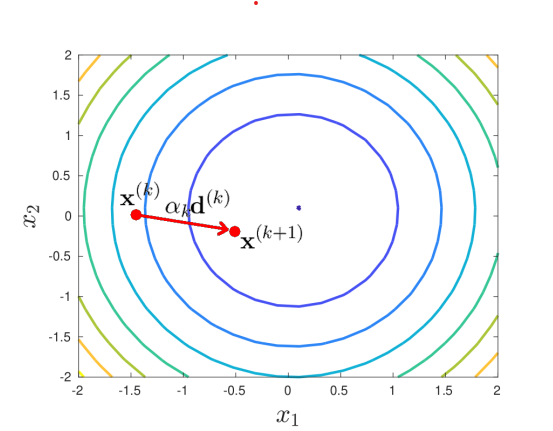
\includegraphics[width=0.5\textwidth]{./img/AnalisiNumerica/gradiente.png}
    \caption{Interpretazione geometrica del metodo del gradiente}
    \label{fig:gradiente}
\end{figure}
Dato che si vuole andare verso il minimo della funzione, l'idea è quella di 
prendere come direzione quella opposta al gradiente. Infatti, il gradiente della 
funzione valutato in un punto restituisce la direzione di massima crescita, la 
direzione opposta corrisponde quindi alla massima decrescita. Fissato $x^{(k)}$,
la direzione di massima decrescita è data da:
\begin{equation}
    d^{(k)} = -\triangledown \phi = b - Ax^{(k)}
\end{equation}
Tale direzione coincide con il residuo al passo $k$, ovvero:
\begin{equation}
    d^{(k)} = r^{(k)} = b - Ax^{(k)}
\end{equation}
Quindi la formula per l'aggiornamento della variabile $x^{(k)}$ diventa:
\begin{equation}
    x^{(k + 1)} = x^{(k)} + \alpha_{k}r^{(k)}
\end{equation}
% ! La parte su come si calcola $\alpha_k$ non è stata fatta a lezione la devo 
% ! aggiungere?
\end{document}